\chapter{StreamingATLOD: Streaming-Assisted Terrain Level of Detail}
%\thispagestyle{fancy} % Apply fancy just to the first page of the chapter if needed
%\thispagestyle{empty}
\fancyhf{}
\lhead[\textit{CHAPTER 4. STREAMINGATLOD}]{}
\rhead[]{\textit{CHAPTER 4. STREAMINGATLOD}}


This chapter describes the implementation of \textit{StreamingATLOD}: \textbf{Streaming-A}ssisted 
\textbf{T}errain \textbf{L}evel \textbf{o}f \textbf{D}etail.
First, some preliminary information, such as 
the used programming languages, tools, libraries, and data will be given.
Afterwards, a high-level overview of StreamingATLOD will be presented.
The missing details from the high-level overview will be filled section 
by section, starting from the main classes and data structures,
followed by geographic conversions, the used meshes, the LOD metric and the culling techniques.
Subsequently, the streaming and caching mechanisms will be presented 
and rounded off with a deep dive into the rendering process, thereby finally filling 
the last piece of missing detail. At the end, a few miscellanous features 
are mentioned, such as the camera, the collision detection and the configuration file support.

\section{Preliminaries}
\subsection{Technologies}
StreamingATLOD is written in C++17 and OpenGL 4.0. For compiling build files,
CMake (minimum version 3.5) is used. The source code of StreamingATLOD 
is hosted on GitHub under the repository \texttt{AmarTabakovic/bachelor-thesis}. StreamingATLOD uses the following third-party
libraries:
\begin{itemize}
  \item GLM: The \textit{OpenGL Mathematics (GLM)} library provides types, functions and constants 
             for the mathematics of computer graphics. It is designed to syntactically ressemble 
             the mathematical features of GLSL, such as vectors, matrices and transforms.
  \item GLEW: The \textit{OpenGL Extension Wrangler} library is an extension loading library for OpenGL.
  \item GLFW: \textit{GLFW} is a multi-platform library for desktop-based OpenGL applications, 
              offering an operating-systems-agnostic API for managing windows, contexts and input handling.
  \item Dear ImGui: \textit{Dear ImGui} is a multi-platform graphical user interface library. StreamingATLOD uses 
          Dear ImGui for a minimalistic user interface.
  \item STB: \textit{STB} is a collection of header-only libraries developed by Sean Barrett. StreamingATLOD uses 
            the header \texttt{stb\_image.h} for loading images.
  \item libwebp: \textit{WebP} is an image format developed by Google designed for images on the web. Its C++ API \textit{libwebp} is used for
                 loading and decoding WebP images.
  \item libcurl: \textit{cURL} is a command-line utility for issuing client-side HTTP-requests. StreamingATLOD uses its 
                  C++ API \textit{libcurl} mainly for downloading the terrain data from web APIs.
\end{itemize}

\subsection{Terrain Data Provider}
The satellite imagery and elevation data is provided by web-based Cloud APIs by the company \textit{MapTiler}.
The datasets ``Satellite V2'' and ``Terrain RGB V2'' are used,
both of which are organized with the XYZ tiling scheme
and projected to Web Mercator. 
The ``Satellite V2'' dataset 
consists of satellite imagery up to zoom level 22 and is served in JPEG format.
The ``Terrain RGB V2'' dataset consists of elevation data up to zoom level 14 and is served in WebP format.
The satellite data will be used up to level 14,
so that there is a 1 to 1 correspondence of satellite tiles and elevation tiles.
Zoom level 14 corresponds to a precision of 9.5 meters per pixel \cite{maptilerzoom}.
This is important for the implemented terrain LOD algorithm, which will be described shortly.

For this thesis, the ``Flex'' plan of MapTiler Cloud was subscribed to,
which costs \$25 per month.
The plan includes 500'000 API requests per month and \$0.10 per 1000 extra requests when exceeding
the monthly 500'000 requests.

The Terrain RGB dataset encodes height values with RGB using a special encoding and decoding formula \cite{maptilerterrainrgb}. The following 
formula converts decodes an RGB triple with each color channel containing values in the range $0,\dots,255$ 
into a height value in meters above sea level:
\begin{align*}
  height = -10000 + ((r \cdot 256^2 + g \cdot 256 + b) \cdot 0.1).
\end{align*}

\subsection{Basic Renderer Design}
The basic renderer design, such as the \texttt{Shader} class and
the structure of the \texttt{Camera} class, 
is based mainly 
on \textit{Learn OpenGL} by de Vries \cite{learnopengl}.
The \texttt{Shader} class represents a single 
OpenGL shader program with a vertex shader and a fragment shader.
It has a field \texttt{unsigned \_id} and various 
methods to set uniform variagles.

The \texttt{Camera} class represents the movable camera and 
is modified slightly in order to allow for better traversal of the Earth.
It will be described in greater detail in section ``Miscellaneous Features''.

\section{System Overview}
This section aims to first outline the terrain LOD algorithm used for StreamingATLOD 
and subsequently give a high-level overview of the system architecture.
The concrete implementation details are described in greater detail in later sections,
slowly filling in the gaps left by the high-level overview.

\subsection{Terrain LOD Algorithm}
The implemented terrain LOD algorithm is mainly based on \textit{Chunked LOD}\cite{chunkedlod}.
Each quadtree node (from now on callled \textit{terrain node} or simply \textit{node}) has either four children or 
no children. Each child node represents a fourth of the parents area 
but at twice the resolution.
The main difference to the original Chunked LOD algorithm is that StreamingATLOD does not 
preprocess the heightmap and compute a TIN per quadtree node. Instead, we 
store a heightmap on each node, upload it to the GPU 
as a texture object and 
use heightmap-displacement in the vertex shader, as described in greater detail 
in sections ``Meshes'' and ``Rendering''.

One major advantage of Chunked LOD is that it maps very straightforwardly to map tiling schemes (in particullar the XYZ tiling scheme), which are also
organized hierarchically. Each terrain node can be uniquely mapped to a satellite overlay tile and a heightmap tile.
Conversely, each satellite tile and heightmap tile can be uniquely mapped to a terrain node.
Additionally, each terrain node can be uniquely identified by its XYZ tile key, which allows for 
constant-time random access using associative data structures such as hashmaps or hashsets,
which will be useful later. Figure \ref{fig:tile-data} 
illustrates this relation between terrain nodes and tiles.

\begin{figure}[H]
  \centering
  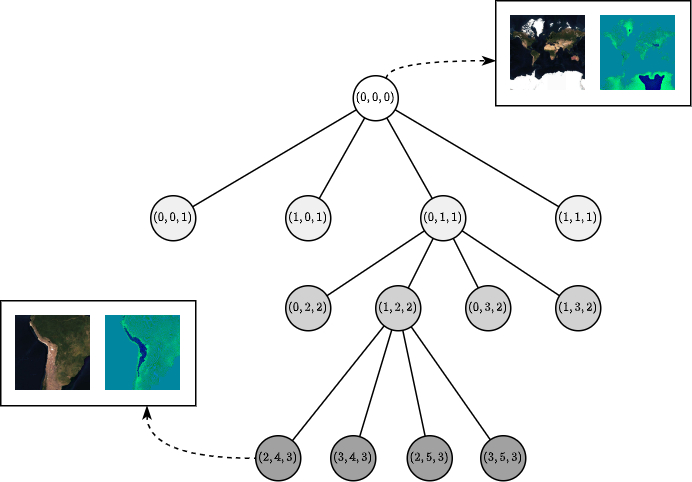
\includegraphics[width=1\textwidth]{tile-key-data.png}
  \caption{A terrain node tree and the associated terrain data (overlay texture and heightmap) that each terrain node stores.}\label{fig:tile-data}
\end{figure}

At runtime, two main steps happen:
\begin{enumerate}
  \item Collection traversal: The first step is the collection of the list of all visible nodes for rendering.
  For this, the terrain nodes get traversed recursively starting from the root node.
  If a traversed terrain node is visible and the traversal should not continue with the node's children,
  the node gets added to the render list. If a node's children are not loaded in memory,
  they get requested and the current node is added to the render list as a replacement.
  \item Rendering: The second step is the actual rendering of the collected visible nodes.
  For this, the list of visible nodes gets iterated and for each node,
  the textures get bound,
  the uniforms get updated and the necessary meshes get rendered.
\end{enumerate}
The details of the rendering process will be described in greater 
detail in section ``Rendering Process''.

\subsection{System Architecture}
StreamingATLOD is built with a multithreaded architecture 
based on worker threads and message queues for inter-thread-communication.
Figure \ref{fig:system-architecture} shows a high-level overview of the system architecture.
The circled numbers are described in the numbered list further below.

\begin{figure}[H]
  \centering
  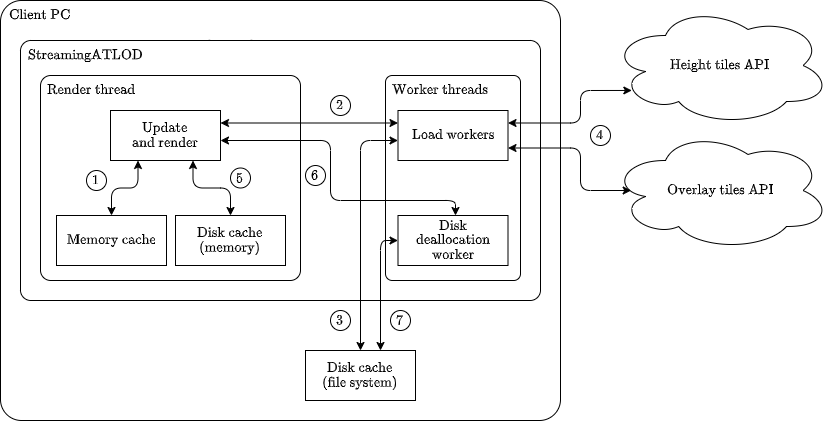
\includegraphics[width=1\textwidth]{system-architecture.png}
  \caption{High-level overview of StreamingATLOD's system architecture.}\label{fig:system-architecture}
\end{figure}

The \textit{render thread} is the main thread where the updating and rendering 
of the terrain happens. It issues all OpenGL commands, including loading various vertex and index buffers at startup,
generating new textures on the GPU, updating uniform variables, performing draw calls and deallocating unused textures from the GPU.
The render thread also manages the \textit{memory cache} and the \textit{disk cache}. 
The memory cache stores all terrain nodes which are  
currently loaded in memory and ready to be rendered. 
The disk cache consists of the \textit{file system disk cache}, which is a folder on the file system that contains the actual heightmaps and overlay images,
and the \textit{in-memory disk cache}, which tracks the tile keys of the data that is stored in the file system disk cache.
Both the memory cache and the disk cache 
are \textit{least-recently used (LRU)} caches with a fixed capacity, which means that 
the least-recently used entries are evicted upon exceeding the capacity. The 
disk cache has a much larger capacity than the memory cache.
The LRU cache implementation will be described in greater detail in section ``Main Classes Data Structures''.

The \textit{worker threads} are separate threads responsible for
tasks that might stall the render thread, such as disk or network I/O.
The main thread and the worker threads communicate with eachother 
through \textit{message passing}. 
Each worker thread has its own \textit{request queue}
for receiving requests, which the main thread can use to send requests
to the worker threads. 
Each worker thread also stores a reference to the main thread's \textit{done queue} for 
sending back responses. Since both the main thread and the worker threads
access the queues, the message queues are \textit{concurrent message queues} which 
lock during each operation for thread-safety. Like the LRU cache implementation, the 
concurrent message queue implementation will be described in greater detail 
in section ``Main Classes and Data Structures'' as well.

There are two types of worker threads employed by StreamingATLOD:
the \textit{load workers}, which load in terrain data from the disk cache 
or from the web APIs, and the single \textit{disk deallocation worker},
which deletes unneeded data from the disk cache.
The terrain nodes in the memory cache and disk cache must be handled 
carefully in order to prevent race conditions and inconsistent application states, such as 
having a terrain node both in the load worker and the disk deallocation worker at the same time.
The implementation details of the worker threads, including the careful handling 
of terrain nodes, is described in greater detail in section ``Terrain Streaming''.

Note that neither worker thread type performs any OpenGL operations, 
since OpenGL calls must happen in the same thread where 
the context is defined \cite{appledevopengl}. Instead, 
all OpenGL operations are performed in the render thread as previously mentioned.

The way that the components and threads work with each other is described in the numbered list below.
The numbers are based on figure \ref{fig:system-architecture}:
\begin{enumerate}[label=\textcircled{\arabic*}]
  \item Each render frame, the visible terrain nodes are traversed and collected for rendering.
        The memory cache stores the most recently used terrain nodes that are ready to be rendered.
        During the collection traversal, we check whether the memory cache contains 
        the desired terrain node, and if so, add it to the list of nodes to be rendered.
        Otherwise, we proceed with \textcircled{2}. Additionally, 
        each render frame we process newly loaded terrain nodes that come off the load worker done queue
        and store them in the memory cache.
  % 2
  \item If during the collection traversal in \textcircled{1} the memory cache did not contain a desired node, 
        the main thread sends a request to a load worker by putting the request 
        on the load worker's request queue.
        Putting a request into the request queue is a non-blocking operation, 
        which means the render thread can continue the collection traversal and rendering. 
        If there are multiple load workers operating, an 
        integer is used to track the load worker which was the most recently used 
        and incremented every time a new request is performed. As a result,
        requests are cyclically distributed over the load workers in a 
        round-robin fashion. The load worker request contains the XYZ tile key of the desired node
        and whether to load the data from the disk cache or from the web API.
        The load worker then processes the request either by retrieving it the heightmap and imagery 
        of the desired node
        from the disk cache \textcircled{3} or from the tile web API \textcircled{4}.
        The load worker also creates the new terrain node object and generates the 
        AABB. Finally, the load worker sends back a response.
        The response can be successful, containing the terrain node instance and, the heightmap and the overlay imagery
        ready to be loaded and rendered.
        It can also send back a failed response, such as when there is a network error 
        or a request timeout, or a so-called \textit{unloadable} response, for when 
        the requested terrain node does not exist (e.g. oceans at high zoom levels).
  % 3
  \item In \textcircled{2} the load worker received a request for loading a terrain node. 
        Based on the request type, the load worker either loads the data 
        from the disk cache on the file system or from the web API.
        In the current numeration, the load worker interacts with the file system cache in two ways.
        The first way is by storing new terrain data that 
        was requested from the web API in the file system disk cache.
        The second way is by reading and loading terrain data from the 
        file system disk cache into memory after the main thread 
        requested them from the disk cache.
  % 4
  \item The load worker communicates with the web APIs after the 
        main thread sent out a request for terrain data from the web APIs. 
        For this, the load worker performs 
        two HTTP requests, one for the heightmap and one for the overlay texture.
        If at least one of both failed, whether due to an error or due 
        to the node being unloadable, the load worker sends back the appropriate 
        response so that the main thread can handle this scenario. 
        Otherwise, the load worker continues constructing the response as described in \textcircled{2}.
  % 5
  \item Every new terrain node that was downloaded from the API gets put into the in-memory disk cache after being 
        processed from the done queue.
        Additionally, during the collection traversal, the in-memory disk cache gets accessed 
        in order to check whether a terrain node is available on the disk cache.
  % 6
  \item Throughout the lifetime of StreamingATLOD, the disk cache grows. Once the maximum 
        capacity has been reached, the least-recently used entries must be evicted from the disk cache.
        This includes deleting the entry from the file system disk cache.
        For this, the render thread sends a request with an XYZ tile key to the disk deallocation worker,
        after which the disk deallocation worker deletes the data from the file system in \textcircled{7}.
        Afterwards, the disk deallocation worker sends a response back to the render thread 
        to signal that it has deleted the data.
  % 7
  \item The disk deallocation worker deletes the actual terrain data on the disk.

\end{enumerate}

\section{Main Classes and Data Structures}
This section describes some of the central classes and data structures used in StreamingATLOD,
starting with the essential XYZ tile key and terrain node classes, followed by the terrain manager class
where the majority of runtime operations happen. Afterwards, the implementation of the two key data structures 
LRU cache and concurrent message queue are described.

\subsection{XYZ Tile Key Class}
The XYZ tile key is represented 
by the class \texttt{XYZTileKey} and is of central importance,
since it is used to identify each terrain node uniquely
and is used as the key type for unordered data structures, such as the \texttt{std::unordered\_map}
or \texttt{std::unordered\_set}. It has three \texttt{unsigned} fields \texttt{\_x},
\texttt{\_y} and \texttt{\_z}. It also contains the four methods 
\texttt{topLeftChild()}, \texttt{topRightChild()},
\texttt{bottomLeftChild()} and \texttt{bottomRightChild()}
to generate each of the four child tile keys.
The \texttt{XYZTileKey} class 
implements a hash function and overrides the 
default comparison function in order to work with 
unordered data structures.

\subsection{Terrain Node Class}
A single terrain node is represented
by the class \texttt{TerrainNode}. The terrain node class serves mainly 
as a simple container and does not include many methods
for runtime behaviour.
Its most important members include the following:
\begin{itemize}
  \item \texttt{XYZTileKey \_tileKey}: The XYZ tile key of the tile.
  \item \texttt{unsigned \_overlayTextureId}: The texture ID of the overlay texture.
  \item \texttt{unsigned \_heightmapTextureId}: The texture ID of the heightmap texture.
  \item \texttt{glm::vec3 \_aabbP1, \_aabbP2}: The two points representing the AABB.
  \item \texttt{std::vector<glm::vec3> \_projectedGridPoints}: The vector containing nine ellipsoid-projected points on the tile arranged in a grid-like manner:
        the top-left, top-center, top-right, middle-left, center, middle-right, bottom-left, bottom-center, bottom-right points.
        These points are used for the LOD metric calculation described in greater detail later.
  \item \texttt{std::vector<glm::vec3> \_horizonCullingPoints}: A vector similar to \texttt{\_projectedGridPoints}, except 
        that the vertices are projected to the ellipsoid using a slightly higher height value. These points 
        are used for horizon culling as described in subsection ``Culling''.
  \item \texttt{unsigned char* \_heightData}: The raw height data. This is used for collision detection.
  \item \texttt{std::chrono::system\_clock::time\_point \_lastUsedTimeStamp}: The timestamp indicating when the tile was last rendered.
\end{itemize}

\subsection{Terrain Manager Class}
The class \texttt{TerrainManager} is the main workhorse of 
StreamingATLOD. All major runtime operations, such as 
updating, rendering, cache management, collision detection and more are performed in 
methods defined in \texttt{TerrainManager}.

The \texttt{TerrainManager} class has numerous members which can be categorized as follows:
\begin{itemize}
  \item Meshes and shaders: The meshes and shaders of the terrain, such as the terrain mesh, skirt mesh and pole mesh,
        are members of \texttt{TerrainManager}, since \texttt{TerrainManager} is responsible for rendering them.
        The mesh types will be introduced in section ``Meshes''.
  \item Caches: \texttt{TerrainManager} holds the memory cache and the in-memory disk cache and also 
                performs the deallocation for evicted for them.
  \item Workers and concurrent message queues: \texttt{TerrainManager} holds the worker thread instances 
        and concurrent message queue instances for the load workers and the disk deallocation worker.
        It also holds the current load worker ID for the round-robin-style load worker scheduling.
  \item Various XYZ tile key lists: The tile keys of terrain nodes that are currently being loaded or that are currently 
        being evicted from the disk are stored on \texttt{std::unordered\_set<XYZTileKey>} instances,
        so that \texttt{TerrainManager} can quickly perform some important checks, e.g. 
        to avoid accidentally requesting a terrain node that is already being loaded or 
        to avoid requesting a terrain node that is currently being evicted from the disk cache.
\end{itemize}

The methods and usage of the member variables will be described in greater detail 
in the subsequent sections wherever they are used.

\subsection{LRU Cache}
The \textit{least-recently used (LRU)} policy is a cache management policy 
which states that only the most-recently used data should be kept.
It is one of many cache management policies used in various areas of 
computer science, such as operating systems, distributed systems and 
web technologies \cite{redislru}.

The \textit{LRU cache} is an associative data structure with a fixed capacity
that operates according to the LRU policy.
Inserting a new key-value pair, updating an existing key-value pair and 
retrieving an existing key-value pair results in the key-value pair 
being the most-recently used and thus the least-likely candidate for eviction.
If the capacity has been reached and a new key-value pair is inserted, 
the least-recently used key-value pair gets evicted.

The LRU cache in StreamingATLOD is implemented as a simple template class \texttt{LRUCache<K,V>},
where \texttt{K} is the key type and \texttt{V} is the value type.
Its capacity can be set in the constructor.
The LRU cache uses a \texttt{std::unordered\_map} and a \texttt{std::list} in the background,
which is a common strategy for implementing LRU caches \cite{redislru}.
It supports the following operations:
\begin{itemize}
  \item \texttt{PutResult<K,V> put(const K\& key, const V\& value)}: This method adds the given key-value pair to the cache.
  If the cache is full, the least-recently used element is evicted and returned as a value of the type \texttt{PutResult<K,V>}.
  The struct \texttt{PutResult<K,V>} stores a \texttt{std::optional<std::}\\ \texttt{-pair<K,V>>}, which either contains the least-recently used key-value pair that was just evicted,
  or \texttt{std::nullopt} if the cache is not full yet. Figure \ref{fig:lru-put-evict} illustrates an example of an eviction after putting a new element into a full cache.
  \begin{figure}[H]
    \centering  
    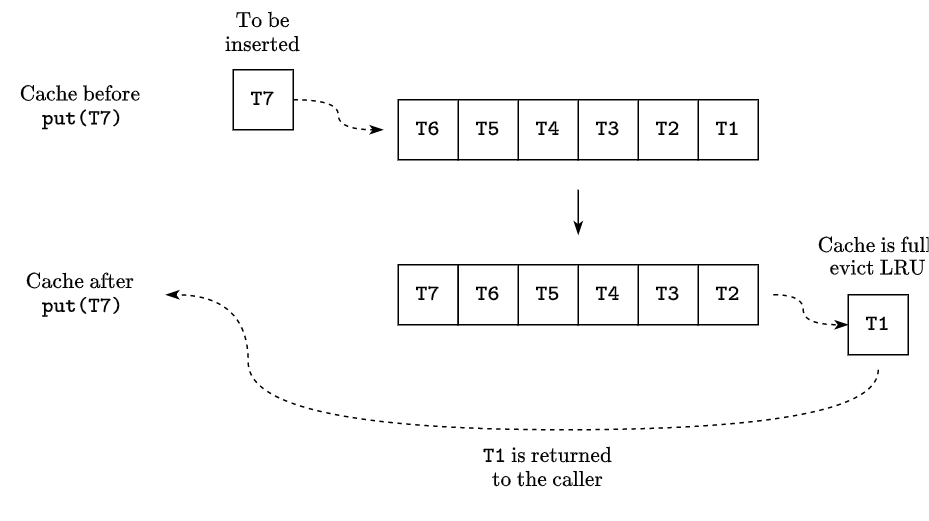
\includegraphics[width=0.85\textwidth]{lru-put-evict.png}
    \caption{Insertion of the element \texttt{T7} with the eviction of the least-recently used element \texttt{T1}.}\label{fig:lru-put-evict}
  \end{figure}
  \item \texttt{std::optional<V> get(const K\& key)}: This method gets the value of the given key. If the value doesn't exist, 
        it returns \texttt{std::nullopt}. Additionally, the cache entry gets pushed to the front of the cache since it was just used.
        Figure \ref{fig:lru-get} illustrates this example.
        \begin{figure}[H]
          \centering  
          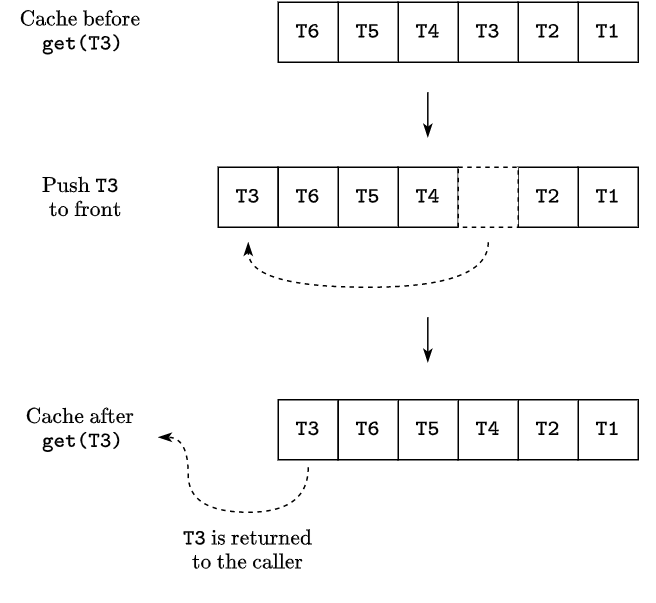
\includegraphics[width=0.65\textwidth]{lru-get.png}
          \caption{Retrieval of the element \texttt{T3}. Note that after the retrieval, \texttt{T3} is the most-recently used element and thus in the front of the cache.}\label{fig:lru-get}
        \end{figure}
  \item \texttt{bool contains(const K\& key)}: This method checks whether an element with a given key exists in the LRU cache without affecting its eviction priority.
\end{itemize}

\subsection{Concurrent Message Queue}
The \textit{concurrent message queue} is a thread-safe data structure designed 
for communicating between different threads. A thread can safely 
push messages to the queue, which can then be processed by another thread.
The access to the queue is locked, such that only a single thread can 
access it at a time. Figure \ref{fig:workers} shows an illustration 
of the concept of using worker threads.

\begin{figure}[H]
  \centering
  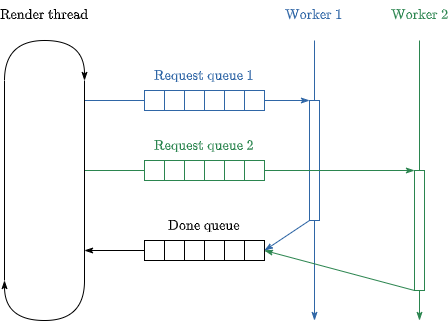
\includegraphics[width=0.75\textwidth]{workers.png}
  \caption{Illustration of the idea of worker threads with message queues. The main thread 
  sends out requests to the request queue, which get processed by the workers in the background and 
  then sent back to the render thread. The image is based on \cite[p.~287]{3denginedesignforvirtualglobes}}\label{fig:workers}
\end{figure}

StreamingATLOD's implementation of
the concurrent message queue is loosely based on 
chapter ``Exploiting Parallelism in Resource Preparation'' in 
the book ``3D Engine Design for Virtual Globes'' by Ring and Cozzi \cite[p.~275]{3denginedesignforvirtualglobes}.

The concurrent message queue is implemented as a small template class \texttt{MessageQueue<T>}.
It supports the following operations, which are all locked using a \texttt{std::mutex} for thread-safety:
\begin{itemize}
  \item \texttt{void push(T message)}: Pushes a message to the concurrent message queue.
  \item \texttt{void pushAll(std::deque<T> messages)}: Pushes the contents of a given queue to the concurrent message queue.
  \item \texttt{std::optional<T> pop()}: Pops and returns the message at the front of the queue. If the queue is empty, \texttt{std::nullopt} is returned.
  \item \texttt{std::deque<T> popAll()}: Pops all messages and returns them in a \texttt{std::deque}.
\end{itemize}

The methods postfixed with \texttt{-All()} allow for quick processing of all elements in 
the queue by a thread without having to repeatedly lock the queue for each element. 

\section{Geographic Conversions}
This section describes the implementation of the main geographic projections and conversions
used in StreamingATLOD. All functions using longitudes and latitudes
expect them in radians as input and return them 
as radians.

The map projections performed on the CPU 
are encapuslated in the C++ header file \texttt{mapprojections.h},
which defines a namespace \texttt{MapProjections}
with functions inside for performing map projections.

\subsection{Web Mercator and Inverse Web Mercator}
The Web Mercator and Inverse Web Mercator projections
are encapsulated in the functions \texttt{webMercator()}
and \texttt{inverseWebMercator()} respectively.
Listing \ref{lst:webmerc} shows the pseudocode 
for both the Web Mercator and the Inverse Web Mercator projections.

\begin{lstlisting}[
  language={C++},
  label={lst:webmerc},
  caption={The functions \texttt{webMercator()} and \texttt{inverseWebMercator()} in \texttt{MapProjections}.}]
inline glm::vec2 webMercator(glm::vec2 lonLat)
{
    float x = (glm::degrees(lonLat.x) + 180.0f) / 360.0f;
    float y = 0.5f - glm::log(glm::tan(glm::pi<float>() / 4.0f + lonLat.y / 2.0f)) / (2.0f * glm::pi<float>());

    return glm::vec2(x, y);
}

inline glm::vec2 inverseWebMercator(glm::vec2 webMercXY)
{
    float lon = glm::radians((webMercXY.x * 360.0f - 180.0f) * -1.0f);
    float lat = glm::radians((glm::atan(glm::exp(glm::pi<float>() * (1.0f - 2.0f * webMercXY.y))) * 2.0f - glm::pi<float>() / 2.0f) * 180.0f / glm::pi<float>());

    return glm::vec2(lon, lat);
}
\end{lstlisting}

\subsection{Geodetic-to-cartesian Transformations}
As mentioned previously, the geodetic-to-cartesian transformations
are based on chapter ``Math Foundations''
of the book ``3D Engine Design for Virtual Globes''
by Cozzi and Ring \cite[p.~13]{3denginedesignforvirtualglobes}.
The first two functions are 
\texttt{geodeticSurfaceNormal()},
which both compute the surface normal on an ellipsoid 
given a geodetic coordinate. The first function takes a 
3D point and the squared ellipsoid radii, whereas the second point 
only takes the squared ellipsoid radii.
The third function is \texttt{toGeodetic2D()},
which computes the 2D geodetic coordinate $(lon,lat)$ given a 3D
cartesian coordinate and the squared ellipsoid radii.
The fourth function is 
\texttt{geodeticToCartesian()},
which given a 2D geodetic coordinate $(lon,lat)$ and 
the squared ellipsoid radii computes the cartesian coordinate on the ellipsoid.
All four functions are shown in listing \ref{lst:geodetic}.

\begin{lstlisting}[
  language={C++},
  label={lst:geodetic},
  caption={The functions \texttt{geodeticSurfaceNormal()}, \texttt{toGeodetic2D()} and \texttt{geodeticToCartesian()} in \texttt{MapProjections}.}]
inline glm::vec3 geodeticSurfaceNormal(glm::vec3 p, glm::vec3 globeRadiiSquared)
{
    glm::vec3 normal = p * (glm::vec3(1.0f) / globeRadiiSquared);
    return glm::normalize(normal);
}

inline glm::vec3 geodeticSurfaceNormal(glm::vec3 geodetic)
{
    float cosLat = glm::cos(geodetic.z);

    return glm::vec3(cosLat * glm::cos(geodetic.x), glm::sin(geodetic.z), cosLat * glm::sin(geodetic.x));
}

inline glm::vec2 toGeodetic2D(glm::vec3 position, glm::vec3 globeRadiiSquared)
{
    glm::vec3 n = geodeticSurfaceNormal(position, globeRadiiSquared);
    return glm::vec2(glm::atan2(n.z, n.x) * -1, glm::asin(n.y / glm::length(n)));
}

inline glm::vec3 geodeticToCartesian(glm::vec3 globeRadiiSquared, glm::vec3 geodetic)
{
    glm::vec3 n = geodeticSurfaceNormal(geodetic);
    glm::vec3 k = globeRadiiSquared * n;
    float gamma = glm::sqrt(k.x * n.x + k.y * n.y + k.z * n.z);

    glm::vec3 rSurface = k / gamma;
    return rSurface + (geodetic.y * n);
}
\end{lstlisting}


\subsection{On the GPU}
The above described functions were implemented in the vertex shaders 
as well where needed. The functions in the shaders are essentially 
the same, except that instead of in C++, they are written in GLSL.
Listing the code for these functions again but in GLSL would be redundant.

\subsection{Choice of Ellipsoid Radii}
As mentioned in ``Theoretical Background'', 
StreamingATLOD does not use the WGS84 ellipsoid with radii $(6378137, 6378137, 6356752.314245)$ for geodetic-to-cartesian conversions.
Instead, it uses an ellipsoid of much smaller scale of $\sqrt{(100000, 100000, 100000)} = (316.2277, 316.2277, 316.2277)$ in order to avoid precision issues.
This value was determined entirely through experimentation, such that there was enough precision for vertex transforms 
and enough precision for the depth buffer.
Since the terrain data is used up to zoom level 14 anyway, which corresponds to a 
maximum precision of around 9.5 meters\cite{maptilerzoom}, specialized solutions for precision issues 
such as the ones described in chapter ``Theoretical Background'' are currently not needed.
Incorporating measures for handling higher precision terrain data is 
a potential improvement point for the future.

\section{Meshes}
This section introduces the three main mesh types used for rendering the Earth: the \textit{terrain mesh},
the \textit{skirt mesh} and the \textit{pole mesh}. Each mesh type 
is encapuslated in its own class (\texttt{GridMesh} for the terrain mesh, \texttt{SkirtMesh} for the skirt mesh 
and \texttt{PoleMesh} for the pole mesh).

\subsection{Terrain Mesh}
StreamingATLOD renders the terrain by displacing the height values of a flat mesh in the vertex shader, 
similarly to GPU-based Geometry Clipmaps \cite{gpugeomclipmaps} and the basic ATLOD\cite{p2}.
This flat mesh, from now on called the \textit{terrain mesh} or \textit{grid mesh},
is a flat square grid-like mesh of side length $n \in \mathbb{N}$ centered around $(0,0,0)$.
Each vertex consists of a $(x,y)$ coordinate and the coordinates go from $(-n,-n)$ to $(n,n)$.
The terrain mesh is organized with triangle strips, so that it can be rendered as the OpenGL \texttt{GL\_TRIANGLE\_STRIP} primitive.
The main advantage of using triangle strips is that they use up less GPU memory in comparison to e.g. \texttt{GL\_TRIANGLES}.
Each row of the mesh is separated with a special marker index named \texttt{RESTART}, which is set 
to the maximum \texttt{GLuint} value. The reason for this is that when starting a new row, 
the indices of the row can be defined immediately after using \texttt{RESTART}, instead of 
the alternative approach of having to 
define so-called \textit{degenerate triangles} in order to start a new row.
Figure \ref{fig:indices} shows an illustration of a $3 \times 3$ terrain mesh.

\begin{figure}[H]
  \centering
  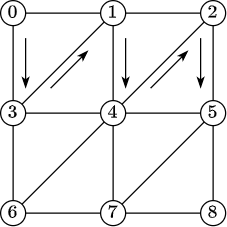
\includegraphics[width=0.35\textwidth]{indices.png}
  \caption{Illustration of a flat $3 \times 3$ terrain mesh viewed from the top. The indices are organized as triangle strips in the following order: 0, 3, 1, 4, 2, 5, \texttt{RESTART}, 3, 6, 4, 7, 5, 8, \texttt{RESTART}.}\label{fig:indices}
\end{figure}

In the vertex shader, the terrain mesh first gets its heights displaced using the heightmap that was loaded on the GPU,
after which it is projected to the ellipsoid with the Inverse Web Mercator projection and the geodetic-to-cartesian transformation.
These operations are described in greater detail in the later section ``Rendering''.

The terrain mesh's side length $n$ can be chosen arbitrarily, since textures can be filtered bilinearly on the GPU.
This also means that the terrain mesh can be defined in multiple resolutions.
StreamingATLOD supports three different terrain mesh side lengths (\texttt{low}, \texttt{medium} and \texttt{high}) 
which can be configured in a configuration file
as described in the later section ``Miscellaneous Features''.
The terrain mesh resolution \texttt{low} is currently rendered for zoom levels 0 to 8,
\texttt{medium} for zoom levels 9 to 11 and \texttt{high} for zoom levels 12 and above.

\subsection{Skirt Mesh}
In order to avoid cracks from occurring StreamingATLOD 
uses skirts as introduced in chapter ``Theoretical Background''.
For this, StreamingATLOD uses a special \textit{skirt mesh}.

The skirt mesh is defined almost exactly the same as the terrain mesh,
having the same side length as the terrain mesh being also organized as triangle strips.
The first main difference is that the skirt mesh only consists of the outermost vertices at the perimeter of the terrain mesh,
whereas the terrain mesh consists of the entire filled  $n \times n$ grid.

The second main difference is that the vertices are defined in a special way.
A skirt mesh vertex consists of a $(x,z)$ coordinate
and additionally a boolean flag indicating whether the current vertex is an \textit{original vertex} or a \textit{skirt vertex}.
An original vertex is a vertex which gets rendered 
in the exact same location as the terrain mesh's corresponding vertex.
A skirt vertex is a vertex whose height will be subtracted by the skirt's height during rendering,
thus forming the skirt.
The skirt height can be chosen arbitrarily, but usually a value slightly larger than the difference between the minimum and maximum
height of the terrain suffices.

In the vertex shader, the scaling, height displacement and ellipsoid transformation occur similarly to the terrain mesh,
but as an additional step, the height of each skirt vertex is subtracted by the skirt height.
In the fragment shader, the texture coordinate is chosen to be at the exact border of the texture,
such that the texture at the border is repeated down the skirt. Figure \ref{fig:skirt} shows an example of a terrain mesh with a skirt mesh.

\begin{figure}[H]
  \centering
  \subfloat[\centering]{{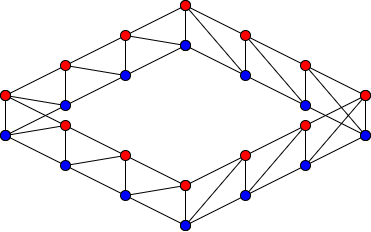
\includegraphics[width=0.45\textwidth]{skirt-vertex.png} }}
  \qquad
  \subfloat[\centering]{{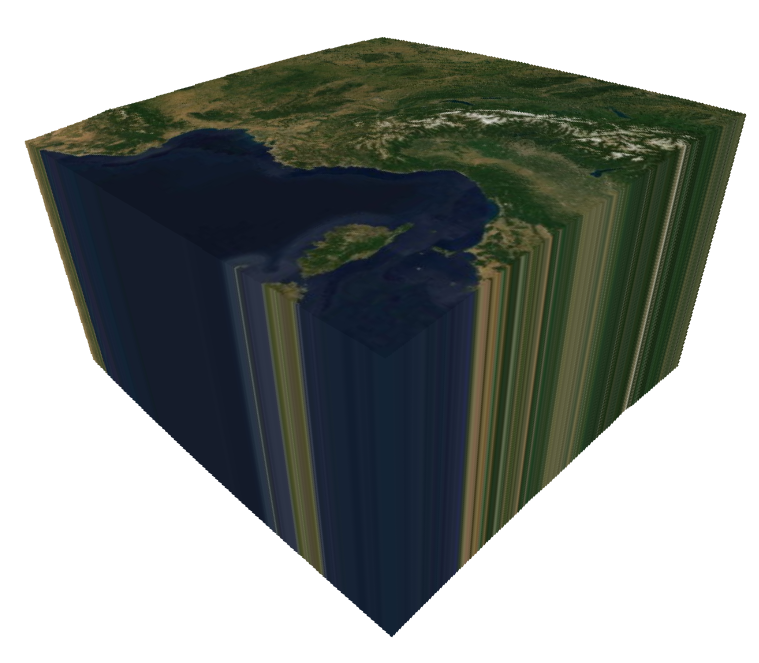
\includegraphics[width=0.4\textwidth]{skirt-terrain.png} }}%
  \caption{Illustration of a skirt mesh with original vertices in red and skirt vertices in blue in subfigure (a) and a rendered terrain node with the skirt in subfigure (b).}\label{fig:skirt}
\end{figure}

\subsection{Pole Mesh}
Recall from chapter ``Theoretical Background'' that the Web Mercator projection cuts off at a latitude of $\pm 85.051129^{\circ}$.
As a result, when rendering the terrain by projecting it to the ellipsoid in the vertex shader, 
a hole appears where the North and South Pole should be. The 
solution is to cover up the hole with another special type of mesh: The \textit{pole mesh}.

The pole mesh, similarly to the terrain and the skirt mesh, is a flat mesh centered around $(0,0,0)$.  
The pole mesh has a single vertex is centered at $(0,0,0)$ and $n_{pole}$ vertices along the circle.
The vertices form a circle with a radius of 1.
The number of vertices along the circle $n_{pole}$ can be programatically defined. StreamingATLOD uses a value of 30.
The vertices are generated by splitting the unit circle into $n_{pole}$ pieces using trigonometry:
\begin{align*}
  \mathbf{p}_i = ({p_i}_x, {p_i}_y) = (\cos(i \cdot (2 \pi / n_{pole})), \sin(i \cdot (2 \pi / n_{pole})))
\end{align*}
for $i \in 0, \dots, n_{pole} - 1$.

Figure \ref{fig:polemesh-wireframe} shows a wireframe render of the pole mesh.

\begin{figure}[H]
  \centering
  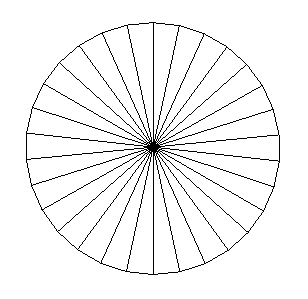
\includegraphics[width=0.55\textwidth]{polemesh-wireframe.png}
  \caption{Wireframe render of the pole mesh viewed from top.}\label{fig:polemesh-wireframe}
\end{figure}

During rendering, the height of the pole mesh is also displaced in the vertex shader, 
but now by an uniform \texttt{float} variable \texttt{earthRadius} 
instead of with a heightmap, since the height of the pole mesh 
is the same everywhere. The uniform \texttt{float} varaible \texttt{isNorthPole} is used 
as a boolean to negate \texttt{earthRadius}, so that both the North and South Pole can be rendered easily.
For scaling the pole mesh in the $x$ and $z$ directions, the uniform variable \texttt{poleRadius} is used.

In the fragment shader, the pole mesh is rendered with a single color, which is either dark blue 
for the North Pole, or white for the South Pole, dependent on \texttt{isNorthPole}.

\section{LOD Metric}
The \textit{LOD metric} determines at what point a terrain node should be split up into its four child nodes.
It gets calculated for every visible node during the collection traversal.
If the metric returns true, the traversal should continue 
with the node's four children, otherwise the traversal ends at the current node.

Recall from subsection ``Main Data Structures'' 
that a terrain node stores 9 points in a grid-like manner in the field \texttt{\_projectedGridPoints}.
The LOD metric function iterates over each point and calculates the distance 
between the camera's position and the current point, as shown in figure \ref{fig:dist-tile}.
If any one of the points lies within a distance threshold, the metric returns true.
If all points lie outside of the distance threshold, the metric returns false.
and the current node is collected to the render list.

\begin{figure}[H]
  \centering
  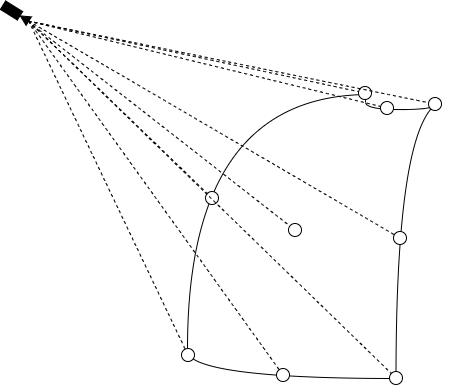
\includegraphics[width=0.55\textwidth]{dist-tile.png}
  \caption{Illustration of calculating the distance between the camera and the 9 projected grid points on the tile.}\label{fig:dist-tile}
\end{figure}

The actual distance threshold is based on a base distance, the current node's zoom level,
and the current node's $y$ tile coordinate. 
The base distance is a predefined constant which represents the distance in world-space units
at which the root node gets split up into its four child nodes.
The node's zoom level is used to scale the base distance down, thus allowing 
the same base distance to be used at every zoom level.
The node's $y$ tile coordinate is used to suppress the splitting of nodes near the North and South Poles.
The reason for this will be made clear in the next few paragraphs.

Recall from chapter ``Theoretical Background'' that the 
latitudes converge towards the North and South Poles, as shown in figure \ref{fig:globe-wireframe}.
The terrain nodes gets smaller and more dense towards the poles compared to other nodes 
with the same zoom level situated closer to the Equator.

\begin{figure}[H]
  \centering
  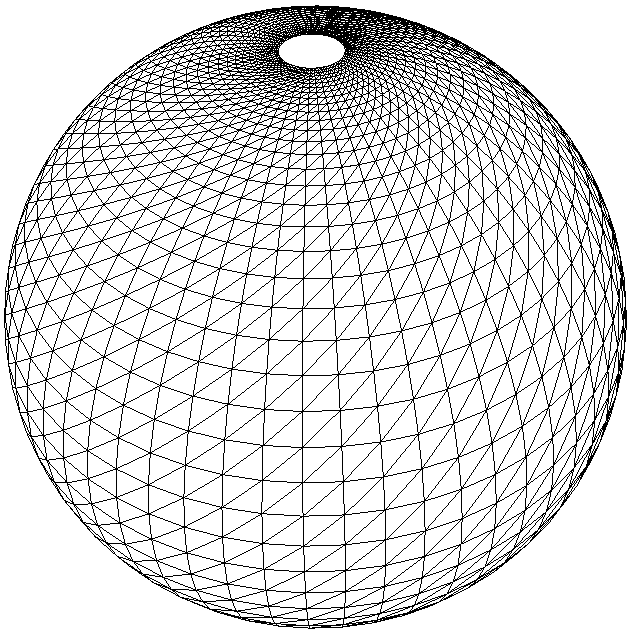
\includegraphics[width=0.35\textwidth]{globe-wireframe.png}
  \caption{Wireframe render of an ellipsoid-projected globe. Notice how the vertices get denser as they approach the North Pole.}\label{fig:globe-wireframe}
\end{figure}

Using the same base distance for all latitudes would result in 
nodes with an unnecessarily high amount of detail being rendered, 
which would not only put a strain on the rendering performance,
since more triangles need to be rendered in a small compressed space,
but also on the streaming performance, since more nodes must be loaded than 
necessary.

The solution to this problem is to reduce 
the base distance using the $y$ tile coordinate of the current node.
The closer a terrain node is to the poles, the lower the base distance will be,
therefore requiring the camera to fly closer to the surface in order to stream 
in and render more detailed nodes near the poles.

In terms of actual values in StreamingATLOD, the base distance is
3.5 times the ellipsoid radius in $x$ direction.
Listing \ref{lst:lod-metric} shows the pseudocode for the split metric.
The values were determined through repeated experimentation.

\begin{lstlisting}[
  language={C++},
  label={lst:lod-metric},
  caption={The methods \texttt{shouldSplit()} and \texttt{computeThresholdWithLatitude()} in \texttt{TerrainManager}.}]
bool TerrainManager::shouldSplit(Camera& camera, XYZTileKey currentTileKey)
{
    float pow2Level = 1 << currentTileKey.z();
    TerrainNode* node = _memoryCache.get(currentTileKey.string()).value();

    // Iterate through grid points, check distance
    for (glm::vec3 point : node->_projectedGridPoints) {
        glm::vec3 cameraToPoint = point - camera.position();
        float cameraDistance = glm::length(cameraToPoint);

        // Latitudes close to the poles should have lower base distance
        float threshold = computeThresholdWithLatitude(currentTileKey);

        // Scale down to appropriate zoom level
        threshold /= pow2Level;

        if (threshold <= cameraDistance)
            return true; // Split the terrain node
    }
    return false; // Do not split the terrain node
}

float TerrainManager::computeThresholdWithLatitude(XYZTileKey tileKey)
{
    // Use globe radius in x direction times 3.5 as base distance (for root node)
    float threshold = GlobalConstants::GLOBE_RADII.x * 3.5;
    float pow2Level = 1 << tileKey.z();

    if (tileKey.z() >= 3 && std::abs(tileKey.y() / pow2Level - 0.5f) >= 0.3)
        threshold *= 0.52;
    else if (tileKey.y() >= 3 && std::abs(tileKey.y() / pow2Level - 0.5f) >= 0.4)
        threshold *= 0.41;

    return threshold;
}
\end{lstlisting}

\section{Culling}
\textit{Culling} refers to the idea of not rendering 
objects that are not visible to the camera and is of special importance
for any rendering system, since it drastically improves the performance 
by reducing the number of triangles that need to be processed by the GPU and rendered.
StreamingATLOD utilizes two culling techniques: \textit{view-frustum culling} and \textit{horizon culling}.

\subsection{View-frustum Culling}
With \textit{view-frustum culling},
objects which lie outside the \textit{view-frustum} do 
not get rendered.
The view-frustum is a three-dimensional pyramid that represents the visible area and is defined by six planes.
Figure \ref{fig:view-frustum-illustration} shows an illustration 
of view-frustum culling with a flat terrain viewed from the top.

\begin{figure}[H]
  \centering
  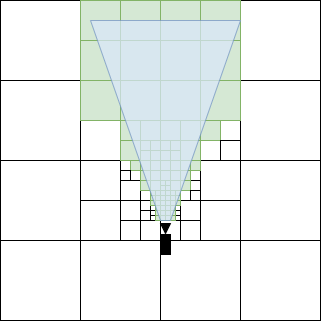
\includegraphics[width=0.55\textwidth]{frustum-culling-illustration.png}
  \caption{Illustration of view-frustum culling with a 
  flat terrain viewed from the top. The blue trapezoid represents 
  the view-frustum and all green nodes are visible and get rendered.}\label{fig:view-frustum-illustration}
\end{figure}

In order to check whether an object, such as a terrain node, is inside the view-frustum, the object 
needs to have a \textit{bounding volume} associated to it.
The bounding volume is simply the volume which contains the entire object inside of it.
There are different types of bounding volumes,
such as \textit{bounding spheres}, \textit{axis-aligned bounding boxes (AABB)}, \textit{oriented bounding boxes (OBB)}, and more,
each with their own strengths and weaknesses. 

In StreamingATLOD, the AABB is chosen as the bounding volume for terrain nodes 
due to its decent balance between accuracy and fast intersection.
While bounding spheres are generally faster to generate and intersect,
they are significantly more inaccurate, often containing large sections of empty space
well above and below the terrain.
OBBs can potentially represent a terrain node more accurately but 
require longer and more complex generation and intersection times.

The usual method of creating a bounding box for a (flat) terrain 
would be to simply combine the minimum and maximum heights with the two extreme corner points (top-left and bottom-right),
$\mathbf{p}_{min}$ and $\mathbf{p}_{max}$.
For a non-flat terrain, however, it gets slightly more complicated.
For zoom levels 0 and 1, simply projecting $\mathbf{p}_{min}$ and $\mathbf{p}_{max}$ from 
the flat terrain to the ellipsoid with the geodetic-to-carteisan transformation does not work.
Consider for example the level 0 root node. Projecting $\mathbf{p}_{min}$ and $\mathbf{p}_{max}$
results in the new points $\mathbf{p'}_{min}$ and $\mathbf{p'}_{max}$ being located at the North and South Pole respectively.
Both projected points have the same longitude, which is $\pm 180^{\circ}$, and 
the resulting AABB is a thin plane which stretches from the North to the South Pole.
The view-frustum intersection test would yield wrong results in many cases 
and occlude sections of the Earth when they should be in reality visible.
Figure \ref{fig:earth-aabb-wrong} visualizes this naive AABB generation method for the root node.

\begin{figure}[H]
  \centering
  \subfloat[\centering]{{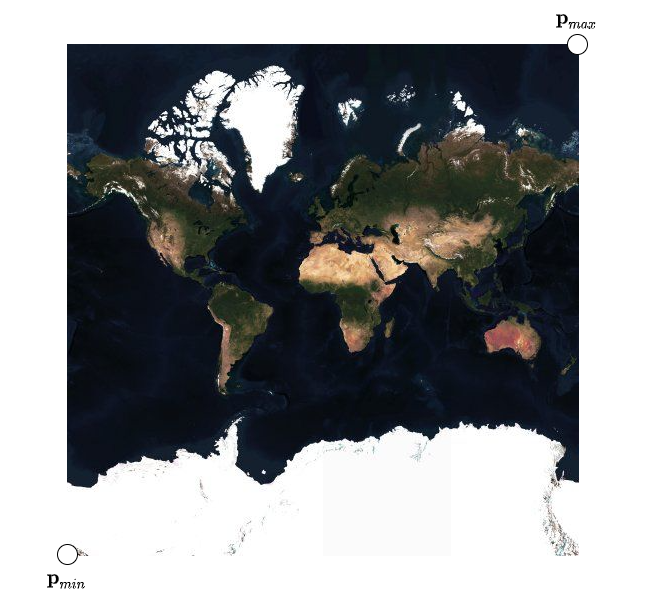
\includegraphics[width=0.5\textwidth]{earth-aabb-0-wrong.png} }}
  \qquad
  \subfloat[\centering]{{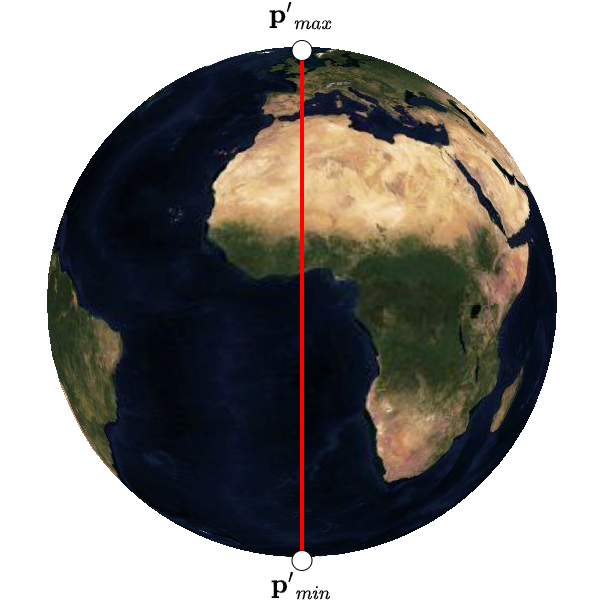
\includegraphics[width=0.4\textwidth]{earth-aabb-1-wrong.png} }}%
  \caption{Naive AABB projection to the ellipsoid for the root node. The points $\mathbf{p}_{min}$ and $\mathbf{p}_{max}$
  get projected onto the poles as shown in subfigure (b).}\label{fig:earth-aabb-wrong}
\end{figure}

To compute the AABB for nodes with zoom level 0, the ellipsoid radii in $(x,y,z)$ directions
$\mathbf{r}_{ellipsoid} = (r_x, r_y, r_z)$ is used. For the zoom level 0 tile, the AABB is generated 
simply by choosing $\mathbf{p}_{min} = -\mathbf{r}_{ellipsoid}$ and 
$\mathbf{p}_{max} = \mathbf{r}_{ellipsoid}$. 

For nodes with zoom level 1, there are four cases: Tile keys $(0,0,1)$, $(1,0,1)$, $(0,1,1)$ and $(1,1,1)$.
Using once again $\mathbf{r}_{ellipsoid}$, the minimum and maximum points $\mathbf{p}_{min}$ and $\mathbf{p}_{max}$ 
are computed by taking the ellipsoid radii such that the 
entire section of the Earth represented by that node lies inside of the two points.
For example, a node with the tile key $(1,0,1)$ (top-right section of the Earth at zoom level 1) gets an AABB with the points 
$\mathbf{p}_{min} = (0,0,-r_z)$ and $\mathbf{p}_{max} = (r_x,r_y,r_z)$.

For nodes with higher zoom levels, the four corner points of the node can now be projected onto the ellipsoid
and the minimum and maximum $(x,y,z)$ coordinates taken from the four projected points.
Each node with zoom level 2 or higher has a minimum and maximum longitude $lon_{min}$ and $lon_{max}$ such that 
$\lvert lon_{max} - lon_{min} \rvert \leq 90^{\circ}$. This means that for nodes with a zoom level 2 or higher, 
the four corner points all lie within the same quarter of any hemisphere, which was not
the case for zoom levels 0 and 1.
Figure \ref{fig:projected-aabb} shows an illustration of an AABB encasing an
ellipsoid-projected terrain node.

\begin{figure}[H]
  \centering
  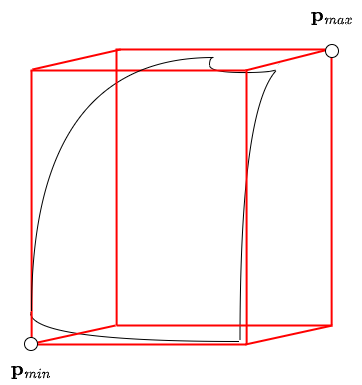
\includegraphics[width=0.55\textwidth]{projected-aabb.png}
  \caption{Illustration of an ellipsoid-projected terrain node with 
  its AABB in red.}\label{fig:projected-aabb}
\end{figure}

StreamingATLOD's view-frustum culling implementation is based on chapter ``Frustum Culling'' in \textit{Learn OpenGL} by de Vries \cite{learnopengl}.
The methods used for view-frustum culling are implemented in the \texttt{Camera} class and shown in listing \ref{lst:frustumculling}.

\begin{lstlisting}[
  language={C++},
  label={lst:frustumculling},
  caption={The methods \texttt{Camera::insideViewFrustum} and \texttt{Camera::checkPlane} for view-frustum culling.}]
bool Camera::insideViewFrustum(glm::vec3 p1, glm::vec3 p2)
{
    Frustum frustum = _viewFrustum;

    unsigned checked = 0;

    checked += checkPlane(frustum.leftFace, p1, p2);
    checked += checkPlane(frustum.rightFace, p1, p2);
    checked += checkPlane(frustum.topFace, p1, p2);
    checked += checkPlane(frustum.bottomFace, p1, p2);
    checked += checkPlane(frustum.nearFace, p1, p2);
    checked += checkPlane(frustum.farFace, p1, p2);

    return checked == 6;
}

bool Camera::checkPlane(Plane& plane, glm::vec3 p1, glm::vec3 p2)
{
    float minY = p1.y;
    float maxY = p2.y;
    float width = p2.x - p1.x;
    float depth = p2.z - p1.z;
    glm::vec3 aabbCenter = p1 + ((p2 - p1) / 2.0f);

    float halfHeight = (maxY - minY) / 2.0f;
    float halfWidth = width / 2.0f;
    float halfDepth = depth / 2.0f;
    float r = halfWidth * std::abs(plane.normal.x)
        + halfHeight * std::abs(plane.normal.y)
        + halfDepth * std::abs(plane.normal.z);

    return -r <= plane.getSignedDistanceToPlane(aabbCenter);
}
\end{lstlisting}

\subsection{Horizon Culling}
View-frustum culling eliminates a large number of nodes which are not visible to the camera, but not all of them.
Consider the following scenario. The camera is above Singapore and looking straight into the ground towards 
the center of the Earth. Intuitively, only the area around Singapore should be rendered. However, the view-frustum also (correctly) intersects 
with the AABB containing the majority of South America, which lies on the opposite side of the Earth, 
resulting in a large section of the Earth being rendered despite not even being visible.
\textit{Horizon culling} solves this problem by omitting nodes which lie beyond the visible horizon from being rendered,
as shown in figure \ref{fig:horizon-culling}.

\begin{figure}[H]
  \centering
  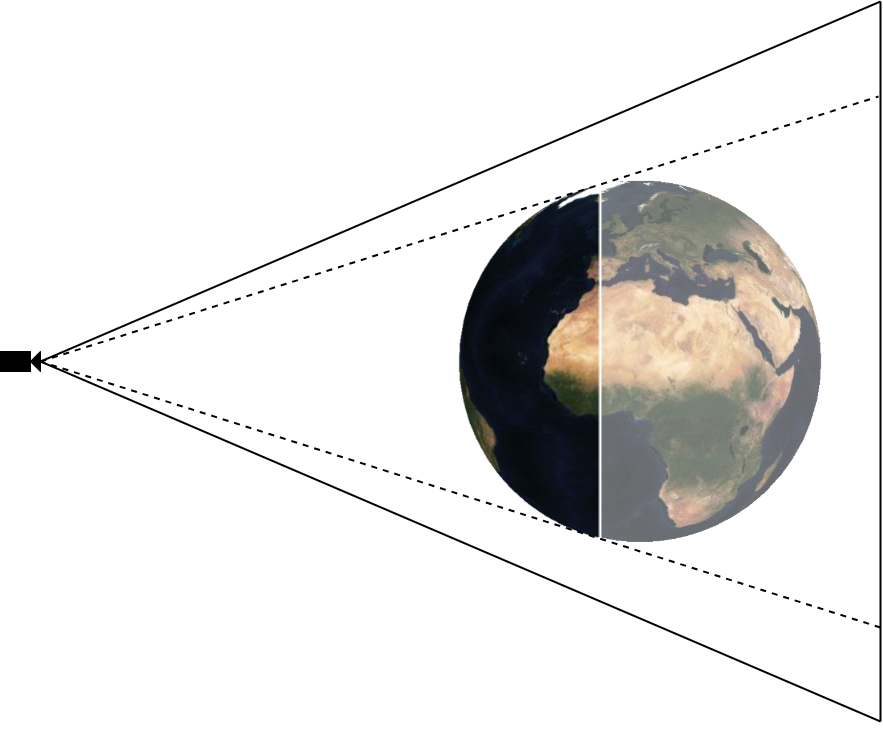
\includegraphics[width=0.65\textwidth]{horizon-culling.png}
  \caption{Illustration of horizon culling. The solid lines represents the view-frustum and the dotted lines are the half-open line segments 
  starting from the camera's position going through the horizon points.}\label{fig:horizon-culling}
\end{figure}

StreamingATLOD's implementation of horizon culling is largely based on the technique described in the
blog article written by Ring at Cesium Geospatial \cite{horizonculling}, which includes a derivation of 
the formulas.
The points for checking against the horizon \texttt{\_horizonCullingPoints} are calculated during the creation 
of the \texttt{TerrainNode*} instance using the node's heightmap, in a similar way 
to the nine \texttt{\_projectedGridPoints}.
The height of each point is set to be slightly higher than the actual 
height value from the heightmap in order to avoid the visual artifact 
of the horizon suddenly popping into view in the distance.
Listing \ref{lst:horizon-culling} shows the pseudocode for checking 
whether a terrain node is horizon culled.

\begin{lstlisting}[
  language={C++},
  label={lst:horizon-culling},
  caption={Method \texttt{horizonCulled()} in \texttt{TerrainNode}.}]
bool TerrainNode::horizonCulled(Camera& camera)
{
    glm::vec3 cv = camera.position() / GlobalConstants::GLOBE_RADII;

    float vhMagnitudeSquared = glm::dot(cv, cv) - 1.0f;

    // Check if all 9 points lie beyond the horizon
    for (auto p : _horizonCullingPoints) {
        glm::vec3 t = p / globeRadius;
        glm::vec3 vt = t - cv;
        float vtMagnitudeSquared = glm::dot(vt, vt);
        float vtDotVc = -1.0f * glm::dot(vt, cv);
        bool isOccluded = vtDotVc > vhMagnitudeSquared && vtDotVc * vtDotVc / vtMagnitudeSquared > vhMagnitudeSquared;

        if (!isOccluded)
            return false;
    }
    return true;
}
\end{lstlisting}

\section{Terrain Caching}
This section describes the caching mechanisms 
for terrain data. As previously mentioned 
in section ``System Overview'', StreamingATLOD uses a
\textit{disk cache} and a \textit{memory cache}.
Both caches are managed as LRU caches with fixed capacities.
Reflected by the fact that computers usually have a much larger disk capacity 
than memory, StreamingATLOD's disk cache 
disk cache is usually much larger than the memory cache.
The cache sizes can be set in the configuration file with the 
requirement that the disk cache is at least 4 times larger than the memory cache.

In addition to LRU, both caches use additional 
special \textit{eviction policies} which specify certain special 
cases for when a least-recently used entry should or should not be evicted.

\subsection{Disk Cache}
The disk cache caches terrain data on the disk 
in order to lower the number of API requests.
The disk cache consists of the \textit{in-memory disk cache}
and the \textit{file system disk cache}.
The in-memory disk cache stores tile keys of terrain nodes whose data is cacjed 
in the file system disk cache. The file system disk cache is a folder
on the client's file system that contains the 
actual heightmap tiles and overlay tiles.

The in-memory disk cache is a field of \texttt{TerrainManager}
named \texttt{\_diskCache} and is 
of the type \texttt{LRUCache<std::string, void*>}.
The value type is \texttt{void*}, since the only required 
information is already in the key.

\subsubsection{Structure of the Disk Cache}
As previously mentioned, the file system disk cache is a folder specified by the user 
on the client's file system.
The folder has two subfolders: the folder \texttt{heightdata},
which stores heightmap tiles, and the folder \texttt{overlay}, which stores 
overlay imagery tiles.
The tiles of both types are stored with the following file name convention:
\texttt{x\_y\_z.ext}, where \texttt{x}, \texttt{y} and \texttt{z}
are the XYZ tile coordinates and \texttt{.ext} is the file extension (\texttt{.jpg} for overlay 
tiles and \texttt{.webp} for heightmap tiles).

\subsubsection{Initialization}
StreamingATLOD needs to know which terrain nodes are already 
cached on the disk.
The method \texttt{TerrainManager::initDiskCache()}, which is executed at start up,
traverses the file system disk cache and collects all file names of the 
tiles in the file system disk cache. 
If there is a heightmap tile that does not have a corresponding 
overlay imagery tile or vice-versa, it gets deleted.
Finally, the XYZ tile key of each collected tile gets 
put into the in-memory disk cache. If the cache's 
capacity is reached during start up, 
the tiles are deleted according to the same eviction policy
used at runtime (see below). 

\subsubsection{Eviction Policy}
The overlay and heightmap with a given XYZ tile key
cannot get evicted from the disk cache if at least one of the following
is true:
\begin{itemize}
  \item It is currently being loaded (i.e. the tile key is in \texttt{\_loadingNodes}).
  \item The current node has at least one child that is cached on the disk as well (i.e. 
  at least one child tile key is in \texttt{\_diskCache}).
  \item The terrain node is the root node.
\end{itemize}
The reason for these limitations is that we always want to evict 
from bottom (high zoom levels) to top (low zoom levels) if possible.

\subsubsection{Putting and Evicting Data at Runtime}
Whenever we process a newly loaded terrain node from the 
load worker done queue \texttt{\_loadDoneQueue} in the method 
\texttt{processAllDoneQueue()} in the main thread, we initialize 
the terrain node in \texttt{initTerrainNode()}.
In \texttt{initTerrainNode()} we also need to insert the tile key of the newly loaded node 
into the in-memory disk cache if it isn't inside of it already and potentially 
evict an old disk cache entry if the disk cache is full.
Listing \ref{lst:initterrainnodedisk} shows the process of doing so 
inside \texttt{initTerrainNode()}.

\begin{lstlisting}[
  language={C++},
  label={lst:initterrainnodedisk},
  caption={Inserting a new in-memory disk cache entry with a potential eviction.}]
void TerrainManager::initTerrainNode() {
    // Initialize node ... 
    // Insert into memory cache ...
    // ... 

    PutResult<XYZTileKey, void*> diskResult = _diskCache.put(tile->xyzTileKey(), nullptr);
    if (diskResult.evicted) {
        XYZTileKey evictedKey = diskResult.evictedItem.value().first;
        // Take the next evicted entry while it does not adhere to the eviction policy
        while (!checkEviction(evictedKey, nullptr) || _loadingTiles.count(evictedKey)) {
            diskResult = _diskCache.put(evictedKey, nullptr);
            evictedKey = diskResult.evictedItem.value().first;
        }
        _currentDiskCacheEvictions.insert(evictedKey);
        _unloadRequestQueue->push({ evictedKey, UNLOAD_REQUEST });
    }
}
\end{lstlisting}
There are four possible cases:
\begin{itemize}
  \item The disk cache is not full and \texttt{\_diskCache} does not contain 
  the tile key of the newly loaded terrain node yet.
  In this case, 
        when putting the tile key in the disk cache, the tile key 
        gets pushed to the front of the in-memory disk cache, making it the most 
        recently-used entry. The \texttt{PutResult}'s \texttt{eviction} flag is 
        set to false in line 7 and disk cache entry gets evicted.
  \item The disk cache is not full and \texttt{\_diskCache} already contains 
        the tile key of the newly loaded terrain node. 
        In this case,
        we proceed indentically as above, except that the cache does not
        have any new entries.
  \item The disk cache is full and \texttt{\_diskCache} contains 
        the tile key for the newly loaded terrain node. 
        Here, we proceed similarly to the previous point, 
        in which the already existing tile key gets pushed 
        to the front without an eviction occurring.
  \item The disk cache is full and \texttt{\_diskCache}
        does not contain the tile key for the newly loaded terrain node. 
        This case is special, since an eviction occurs which needs to 
        be handled. We first check whether we are allowed to 
        evict the entry by entering the while loop condition check
        in line 10. If the entry can be evicted, we skip 
        the while loop's body, track the tile key as being currently 
        evicted in \texttt{\_currentDiskCacheEvictions} and proceed to send 
        a request to the disk deallocation worker request queue (lines 14 and 15).
\end{itemize}

The while loop (lines 10 to 13) may seem problematic at first,
since it bypasses the LRU policy by reinserting a 
least-recently used item back to the front of the cache.
Also, at first sight there might seem like a risk of long waiting times in the while loop
if there are many entries towards the end of the cache 
that cannot be evicted. However, in practice, these points 
are not as problematic as they seem. When a least-recently used entry
is checked for whether it can be evicted and it turns out it cannot be,
it makes the most sense to put it in the front of the cache, 
since want to check all other nodes for eviction.
Also, the problem of long waiting times in the while loop is unlikely.
The collection traversal occurs top-down (from low zoom levels to high zoom levels) and 
when the camera flies from one place to another, terrain nodes further up the in the quadtree 
are likely traversed again throughout subsequent render frames, as shown in figure \ref{fig:eviction-quadtree}.
As a result, the entries towards 
the end of the cache tend to be nodes with high zoom levels with likely 
few child nodes, if at all.

\begin{figure}[H]
  \centering
  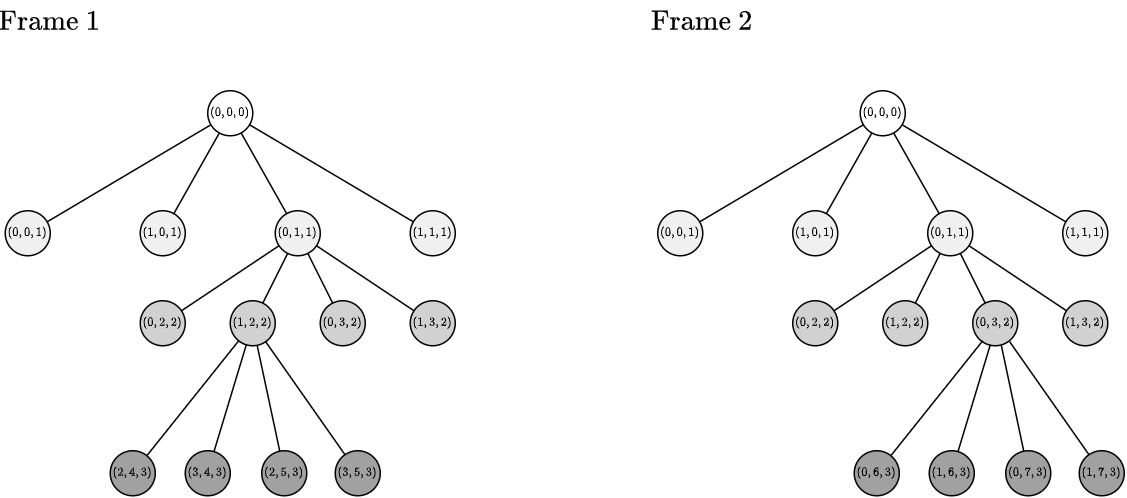
\includegraphics[width=1\textwidth]{eviction-quadtree.png}
  \caption{Illustration of a terrain node tree in a first and a second render frame.
  The nodes further up in the hierarchy are more likely to be used in 
  throughout subsequent frames than nodes further down.}\label{fig:eviction-quadtree}
\end{figure}

\subsubsection{Disk Deallocation Worker}
The disk deallcation worker is the worker thread that performs 
the actual deletion of terrain tiles on the file system disk cache
and is represented by the class \texttt{DiskDeallocationWorkerThread}.
The \texttt{TerrainManager} manages it and stores a \texttt{DiskDeallocationWorkerThread \_unloadWorkerThread},
a \texttt{MessageQueue<DiskDeallocationRequest>* \_unloadRequestQueue} for sending requests , 
\texttt{MessageQueue<DiskDeallocationResponse>* \_unloadDoneQueue} for receiving responses and 
a \texttt{std::unordered\_set<XYZTileKey> \_currentDiskCacheEvictions} for tracking 
entries that are currently being deallocated from the disk.

\subsection{Memory Cache}
The memory cache is the main storage for 
terrain nodes which are currently loaded in memory and ready 
to be rendered. The memory cache is stored
as the field \texttt{LRUCache<std::string, TerrainNode*> \_memoryCache} of the \texttt{TerrainManager}
class.

\subsubsection{Eviction Policy}
The additional eviction policies for the memory cache are almost identical 
to the disk cache, except we do not check whether 
the data is currently being loaded, since it already 
is loaded in memory. 

\subsubsection{Putting and Evicting Data at Runtime}
The eviction happens almost 
identically to the disk cache's eviction shown in listing \ref{lst:initterrainnodedisk},
except that we destroy the \texttt{TerrainNode*} instance and its associated 
OpenGL texture objects directly in the main thread, rather 
than on a separate deallocation thread. 

\section{Terrain Streaming}
This section dives into the multithreaded streaming mechanism 
of StreamingATLOD. For this, the section will mainly resolve 
around the load worker thread, which is responsible for loading 
data in the background. 

\subsection{Load Worker Thread}
The load worker thread is encapsulated in the class \texttt{LoadWorkerThread},
as shown in listing \ref{lst:loadworkerclass}.

\begin{lstlisting}[
  language={C++},
  label={lst:loadworkerclass},
  caption={The class \texttt{LoadWorkerThread}.}]
class LoadWorkerThread
{
public:
    LoadWorkerThread(MessageQueue<LoadRequest>* requestQueue, MessageQueue<LoadResponse>* doneQueue);

    void postRequest(XYZTileKey tileKey);
    void startInAnotherThread();
    void run();

    void processAllRequests();
    void fetchOverlay(LoadRequest& request, LoadResponse& response);
    void fetchHeightmap(LoadRequest& request, LoadResponse& response);

    void loadHeightmapFromDisk(LoadRequest& request, LoadResponse& response);
    void loadOverlayFromDisk(LoadRequest& request, LoadResponse& response);
    void loadHeightmapFromApi(LoadRequest& request, LoadResponse& response);
    void loadOverlayFromApi(LoadRequest& request, LoadResponse& response);

    MessageQueue<LoadRequest>* _requestQueue;
    MessageQueue<LoadResponse>* _doneQueue;

    std::thread _thread;
    CURL* _curl;
    bool _stopThread = false;
};
\end{lstlisting}

Its members are the request queue and the done queue,
the \texttt{std::thread} instance,
the \texttt{CURL} handle for loading tiles from the web APIs,
and the boolean flag that indicates whether the thread 
should be stopped. The cURL handle is defined as a member 
in order to be able to reuse it over multiple requests, which improves 
performance \cite{curlhandlereuse}.

\subsubsection{Load Request and Response Types}
The load worker request and done queues hold values of the struct types \texttt{LoadWorkerRequest}
and \texttt{LoadWorkerResponse} respectively. 

The struct \texttt{LoadWorkerRequest},
shown in listing \ref{lst:loadrequeststruct}
contains the tile key that should be loaded and an enum \texttt{LoadRequestType}
indicating whether to load from the disk cache or from the web API.
\begin{lstlisting}[
  language={C++},
  label={lst:loadrequeststruct},
  caption={The struct \texttt{LoadRequest} and enum \texttt{LoadRequestType}.}]
enum LoadRequestType {
    LOAD_REQUEST,
    LOAD_REQUEST_DISK_CACHE,
    LOAD_STOP_THREAD
};

struct LoadRequest {
    XYZTileKey tileKey;
    LoadRequestType type;
};
\end{lstlisting}

The struct \texttt{LoadWorkerResponse},
shown in listing \ref{lst:loadresponsestruct}
contains the enum \texttt{LoadResponseType} as a return code 
for the main thread, the newly created \texttt{TerrainTile*},
heap-allocated \texttt{unsigned char} pointers to the raw heightmap and overlay texture
and their image dimensions,
and an enum \texttt{LoadResponseOrigin} indicating whether the data 
was loaded from the disk cache or from the web API.
The raw data pointers will be deallocated in the main 
thread when they are not needed anymore.

\begin{lstlisting}[
  language={C++},
  label={lst:loadresponsestruct},
  caption={The struct \texttt{LoadResponse}, enum \texttt{LoadResponseOrigin} and enum \texttt{LoadResponseType}.}]
enum LoadResponseType {
    LOAD_OK, // Loaded alright 
    LOAD_ERROR, // Network error
    LOAD_UNLOADABLE, // No error, but tile does not exist, e.g. oceans at high zoom levels
    LOAD_TIMEOUT, // Web API timed out due to e.g. rate limiting
    LOAD_STOPPED_THREAD // Signal for stopping the worker thread
};

enum LoadResponseOrigin {
    LOAD_ORIGIN_DISK_CACHE,
    LOAD_ORIGIN_API
};

struct LoadResponse {
    LoadResponseType type;
    TerrainNode* tile;
    unsigned char* heightData;
    unsigned char* overlayData;
    unsigned heightmapWidth;
    unsigned heightmapHeight;
    unsigned overlayWidth;
    unsigned overlayHeight;
    LoadResponseOrigin origin;
};
\end{lstlisting}

\subsection{Load Worker Request Queue Processing}
The method \texttt{startInAnotherThread()}
starts the load worker thread in another thread and 
starts the listening loop, which continually calls 
the method \texttt{processAllRequests()} until 
the thread should be stopped.
The method \texttt{processAllRequests()} is responsible for processing
messages coming in on the request queue and is shown 
in listing \ref{lst:processallrequests}.

\begin{lstlisting}[
  language={C++},
  label={lst:processallrequests},
  caption={The method \texttt{LoadWorkerThread::processAllRequests()}.}]
void LoadWorkerThread::processAllRequests()
{
    auto requests = _requestQueue->popAll();

    bool returnNetworkErrors = false;

    for (auto request : requests) {
        if (request.type == LOAD_STOP_THREAD)
            _stopThread = true;
        
        LoadResponse response = { LOAD_OK, request.tileKey, nullptr, nullptr, nullptr, 0, 0, 0, 0, 0, LOAD_ORIGIN_DISK_CACHE };

        if (returnNetworkErrors) {
            response.type = LOAD_ERROR;
            _doneQueue->push(response);
            continue;
        }

        fetchHeightmap(request, response);

        if (response.type != LOAD_OK) {
            if (response.type == LOAD_ERROR)
                returnNetworkErrors = true;
            _doneQueue->push(response);
            continue;
        }

        fetchOverlay(request, response);

        if (response.type != LOAD_OK) {
            if (response.type == LOAD_ERROR)
                returnNetworkErrors = true;
            _doneQueue->push(response);
            continue;
        }

        if (response.type == LOAD_OK) {
            TerrainNode* newTile = new TerrainNode(request.tileKey);
            newTile->_heightData = response.heightData;

            newTile->generateMinMaxHeight();
            newTile->generateAabb();
            newTile->generateProjectedGridPoints();
            newTile->generateHorizonPoints();

            response.tile = newTile;
        }

        _doneQueue->push(response);
    }

    // Respond to main thread that we have stopped the thread
    if (_stopThread)
        _doneQueue->push({ LOAD_THREAD_STOPPED, request.tileKey, nullptr, nullptr, nullptr, 0, 0, 0, 0, 0, LOAD_ORIGIN_DISK_CACHE });
}
\end{lstlisting}

When processing the request queue, the method first 
pops all messages off the request queue (line 3) and loads first 
the heightmap (line 19) and then the overlay (line 28).
If the heightmap failed loading, then we preemptively 
send back a response with a failure response type without 
loading the overlay texture (lines 13 to 17), since we cannot render 
a terrain node if at least one of them is unavailable. The same 
occurs if the heightmap succeeded loading but 
the overlay failed (lines 30 to 36).
The reason for sequentially loading the heightmap 
and the overlay image is to reduce the number 
of requests in case of an error or an unloadable tile,
since we preemptively stop processing the request 
as soon as the heightmap loading fails.

If the response type is \texttt{LOAD\_UNAVAILABLE} or 
\texttt{LOAD\_TIMEOUT},
then we simply send back the response with that code.
If the response type is \texttt{LOAD\_ERROR},
then something must be wrong with the network connection,
which we have to handle specially. We first 
set \texttt{returnNetworkErrors} to true (lines 23 and 32),
which causes all subsequent requests to be 
responded to with responses of the type \texttt{LOAD\_ERROR} (lines 13 to 17).
These responses will signal to the main thread that 
it should wait for a short amount of time before 
sending new web API requests. 

If the main thread signalled to the load worker that it should stop 
running by sending a request of the type \texttt{LOAD\_STOP\_THREAD}, for example when the application shuts down, 
the load worker sets its member flag \texttt{\_stopThread} to true (line 8 and 9)
and finishes procesing all remaining requests,
after which it sends a response of the main thread 
of the type \texttt{LOAD\_THREAD\_STOPPED}.

\subsection{Overlay and Heightmap Loading}
The methods \texttt{fetchOverlay()} and \texttt{fetchHeightmap()}
are responsible for loading the overlay and heightmap of a terrain node respectively.
Both functions take mutable references to 
the requests and responses defined in the method \texttt{processAllRequests()}.
At the end of both function calls, the \texttt{response} variable in the caller 
should contain all relevant information, such as terrain data, 
response code and the origin of the response (disk or API).
Both functions are shown in listing \ref{lst:loadoverlayheightmap}.

\begin{lstlisting}[
  language={C++},
  label={lst:loadoverlayheightmap},
  caption={The methods \texttt{loadOverlay()} and \texttt{loadHeightmap()}.}]
void LoadWorkerThread::fetchHeightmap(LoadRequest& request, LoadResponse& response)
{
    if (request.type == LOAD_REQUEST_DISK_CACHE) { // Load from disk
        loadHeightmapFromDisk(request, response);
        response.origin = LOAD_ORIGIN_DISK_CACHE;
    } else if (!request.offlineMode) { // Load from API if not offline
        loadHeightmapFromApi(request, response);
        response.origin = LOAD_ORIGIN_API;
    } else // Offline mode, we cannot request new tiles
        response.type = LOAD_UNLOADABLE;
}

LoadWorkerThread::fetchOverlay(LoadRequest& request, LoadResponse& response)
{
    if (request.type == LOAD_REQUEST_DISK_CACHE) {
        loadOverlayFromDisk(request, response);
        response.origin = LOAD_ORIGIN_DISK_CACHE;
    } else if (!request.offlineMode) {
        loadOverlayFromApi(request, response);
        response.origin = LOAD_ORIGIN_API;
    } else // Offline mode, we cannot request new tiles
        response.type = LOAD_UNLOADABLE;
}
\end{lstlisting}

Both functions work very similarly. If the request 
for the terrain data is of the type \texttt{LOAD\_REQUEST\_DISK\_CACHE},
then it means that the in-memory disk cache in the main thread 
contains the required entry and we can load the data from the file system disk cache 
into memory in the load worker thread.

\subsection{Loading Data from the Disk Cache}
The process for loading the overlay texture and the 
heightmap texture is essentially identical, except 
for the fact that the overlay image format is JPG 
and that the heightmap image format is WebP.
For this reason, in this and the next subsections 
discussing the loading process, we will only look 
at the loading process for the overlay texture 
in order to avoid redundant explanations.

The method \texttt{loadOverlayFromDisk()} simply 
loads the overlay image from the file system disk cache using 
the disk cache path specified in the configuration file (see Section ``Additional Features'').
This method should not be able to fail, 
since the in-memory disk cache indicated 
that the overlay image is in the file system disk cache.
Inn the exceptional case that it does fail, 
we simply mark it as unloadable. 
Listing \ref{lst:loadoverlayfromdisk} shows the method \texttt{loadOverlayFromDisk()}.

\begin{lstlisting}[
  language={C++},
  label={lst:loadoverlayfromdisk},
  caption={The method \texttt{LoadWorkerThread::loadOverlayFromDisk}.}]
void LoadWorkerThread::loadOverlayFromDisk(LoadRequest& request, LoadResponse& response)
{
    XYZTileKey tileKey = request.tileKey;
    int width, height, nrChannels;
    std::string fileName = ConfigManager::getInstance()->diskCachePath()
        + "overlay/" + std::to_string(tileKey.x()) 
        + "_" + std::to_string(tileKey.y()) 
        + "_" + std::to_string(tileKey.z()) + ".jpg";

    unsigned char* data = stbi_load(fileName.c_str(), &width, &height, &nrChannels, 0);

    if (data) {
        response.overlayData = data;
        response.overlayWidth = width;
        response.overlayHeight = height;
        response.type = LOAD_OK;
    } else {
        std::cerr << "Failed opening overlay texture from cache " << tileKey.string() << std::endl;
        response.type = LOAD_UNLOADABLE;
    }
}
\end{lstlisting}

\subsection{Loading Data from the Web API}
The method \texttt{loadOverlayFromApi()}
loads the overlay and is shown in listing \ref{lst:loadoverlayfromapi}.

\begin{lstlisting}[
  language={C++},
  label={lst:loadoverlayfromapi},
  caption={The method \texttt{loadOverlayFromApi()}.}]
void LoadWorkerThread::loadOverlayFromApi(LoadRequest& request, LoadResponse& response)
{
    XYZTileKey tileKey = request.tileKey;

    std::string responseData;
    std::string url = ConfigManager::getInstance()->overlayDataServiceUrl()
        + std::to_string(tileKey.z()) + "/"
        + std::to_string(tileKey.x()) + "/"
        + std::to_string(tileKey.y()) + ".jpg?key=" + ConfigManager::getInstance()->overlayDataServiceKey();

    if (!_curl) { // Curl handle failed
        std::cerr << "Curl failed" << std::endl;
        std::exit(1);
    }

    curl_easy_setopt(_curl, CURLOPT_URL, url.c_str());
    curl_easy_setopt(_curl, CURLOPT_WRITEFUNCTION, writeData);
    curl_easy_setopt(_curl, CURLOPT_WRITEDATA, &responseData);
    curl_easy_setopt(_curl, CURLOPT_TIMEOUT, 5L); // Timeout is after 5 seconds

    int httpStatusCode = 0;
    int retCode = curl_easy_perform(_curl);

    // Timeout occurred
    if (retCode == CURLE_OPERATION_TIMEDOUT) {
        std::cout << "Heightmap timeout" << std::endl;
        response.type = LOAD_TIMEOUT;
        return;
    }

    // Get HTTP status code
    curl_easy_getinfo(_curl, CURLINFO_RESPONSE_CODE, &httpStatusCode);

    if (retCode != CURLE_OK) { // Network error
        std::cerr << "Network error" << std::endl;
        response.type = LOAD_ERROR;
        return;
    } else if (httpStatusCode == 204) { // Unloadable tile, e.g. oceans at high zoom levels
        std::cerr << "Tile is empty" << std::endl;
        response.type = LOAD_UNLOADABLE;
        return;
    } else if (httpStatusCode != 200) { // Something else went wrong in the API
        std::cerr << "Status code " << httpStatusCode << " in loading overlay" << std::endl;
        response.type = LOAD_ERROR;
        return;
    }

    int width, height, nrChannels;
    unsigned char* data = stbi_load_from_memory((unsigned char*)responseData.c_str(), responseData.size(), &width, &height, &nrChannels, 0);
    if (data) {
        std::string filePath = ConfigManager::getInstance()->diskCachePath() + "overlay/"
            + std::to_string(tileKey.x()) + "_"
            + std::to_string(tileKey.y()) + "_"
            + std::to_string(tileKey.z()) + ".jpg";
        std::ofstream file(filePath, std::ios::out | std::ios::binary);
        if (file.is_open()) {
            file.write(responseData.c_str(), responseData.size());
            file.close();
        } else { // Couldn't open new file for texture image, something severly went wrong
            std::cerr << "Failed to open file for writing." << std::endl;
            std::exit(1);
        }

        response.overlayData = data;
        response.overlayWidth = width;
        response.overlayHeight = height;
        response.type = LOAD_OK;
    } else { // Couldn't decode overlay texture image, something severly went wrong
        std::cerr << "Failed opening overlay texture" << std::endl;
        std::exit(1);
    }
}
\end{lstlisting}
As a first step, it builds the request URL using the URL and 
API key set in the configuration (lines 3 to 9). Afterwards, it checks 
whether the cURL handle is valid (lines 11 to 14) and if so, sets 
the request options, such as the URL, 
the write function, the response buffer
and the maximum time before timeout (lines 16 to 19).
Then, it performs the actual cURL HTTP request (line 22).
First, we check whether the HTTP request timed out and if so, we 
set our response to \texttt{LOAD\_ERROR} and return (lines 24 to 29).
Otherwise, we retrieve the HTTP status code (line 32) and 
check for various conditions, such as whether a network 
error occurred (lines 34 to 37), the tile is unloadable (lines 38 to 41),
or whether the web API responded with a HTTP status code $\neq 200$ (lines 42 to 45).
If none of these conditions were true, we load decode the overlay image 
using \texttt{stbi\_load\_from\_memory()} (line 49) and 
store the image to the file system disk cache (lines 51 to 58).
As a final step, we set the response struct members
to contain the raw decoded overlay image data, the width and height of the overlay image 
and set the response type to \texttt{LOAD\_OK} (lines 64 to 67).

\subsection{Processing New Nodes in the Render Thread}
As previously mentioned, the render thread performs two main operations 
of collecting the terrain nodes to be rendered and rendering them.
But before performing these two operations, it processes new 
messages from the various worker thread queues.
The method \texttt{TerrainManager::processAllLoadDoneQueue()} 
retrieves and processes all elements from the load worker done queue 
and is shown in listing \ref{lst:processalldonequeue}.

\begin{lstlisting}[
  language={C++},
  label={lst:processalldonequeue},
  caption={The method \texttt{LoadWorkerThread::processAllDoneQueue()}.}]
void TerrainManager::processAllDoneQueue()
{
    std::deque<LoadResponse> responses = _doneQueue->popAll();

    for (auto response : responses) {
        // Finished loading, do not need to track anymore
        _loadingNodes.erase(response.tileKey);

        // Handle potential errors or unloadable tiles
        if (response.type == LOAD_UNLOADABLE || response.type == LOAD_TIMEOUT || response.type == LOAD_ERROR) {
            // Unloadable node, store it in unloadable set to prevent future requests
            if (response.type == LOAD_UNLOADABLE)
                _unloadableTileKeys.insert(response.tileKey);

            // Network error, wait for 5 seconds before starting new request
            if (response.type == LOAD_ERROR) {
                _lastNetworkError = std::chrono::system_clock::now();
                _offlineWait = true;
            }

            if (response.heightData != nullptr) {
                delete[] response.heightData;
            }
            if (response.overlayData != nullptr) {
                stbi_image_free(response.overlayData);
            }

            delete response.node;
            continue;
        } else
            initTerrainNode(response);
    }
}
\end{lstlisting}
We first pop all entries from the load worker done queue 
(line 3). Afterwards, we iterate all popped entries  
and first remove the entry of the tile key from 
the set of tile keys whose nodes are being loaded (line 7).
Next, we check whether we received an error or an unloadable 
node (line 10) and check the following two cases:
\begin{itemize}
  \item If the node is unloadable, then we put it in the set of 
        unloadable nodes \texttt{\_unloadableTileKeys} (lines 12 and 13)
        to avoid requesting it again in the future.
  \item If the response was an error, we update the 
        timestamp that indicates when the last error occurred \texttt{\_lastNetworkError}
        to the current time (line 17) and and set the 
        flag \texttt{\_offlineWait} to true (line 18),
        indicating that we should wait a few seconds before 
        requesting new data from the web APIs.
\end{itemize}
Finally, we delete the data of the terrain node (lines 21 to 28)
and continue with the next entry (line 29).

If no error occured, we simply continue processing the terrain node 
in \texttt{TerrainManager::initTerrainNode()}.

In it, we generate the OpenGL texture objects for 
the heightmap and overlay that we just received
and put the node's tile key in the memory cache
and the disk cache if it was loaded from the web API.

The overlay textures additionally get generated with mipmaps for 
trilinear filtering in order to reduce aliasing artifacts in the distance.
Since the textures always have a width and height of 512 pixels, which is a power of two,
mipmap generation occurs quickly and should not significantly hinder rendering performance.
It also comes with an additional GPU memory overhead of only 33\%.
Both textures are clamped in order to avoid
texture artifacts due to limited texture coordinate precision 
at the border of the textures.
Listing \ref{lst:texturegen} shows the OpenGL texture generation pseudocode.

\begin{lstlisting}[
  language={C++},
  label={lst:texturegen},
  caption={OpenGL texture generation for the overlay and the heightmap in \texttt{initTerrainNode()}.}]
void TerrainManager::initTerrainNode(LoadResponse response) {
    TerrainNode* node = response.node;

    // Overlay texture
    glGenTextures(1, &node->overlayTextureId);
    glBindTexture(GL_TEXTURE_2D, node->overlayTextureId);

    glTexParameteri(GL_TEXTURE_2D, GL_TEXTURE_WRAP_S, GL_CLAMP_TO_EDGE);
    glTexParameteri(GL_TEXTURE_2D, GL_TEXTURE_WRAP_T, GL_CLAMP_TO_EDGE);
    glTexParameteri(GL_TEXTURE_2D, GL_TEXTURE_MIN_FILTER, GL_LINEAR_MIPMAP_LINEAR);
    glTexParameteri(GL_TEXTURE_2D, GL_TEXTURE_MAG_FILTER, GL_LINEAR);

    glTexImage2D(GL_TEXTURE_2D, 0, GL_RGBA, overlayWidth, overlayHeight, 0, GL_RGB, GL_UNSIGNED_BYTE, overlayData);
    glGenerateMipmap(GL_TEXTURE_2D);

    // Heightmap texture
    glGenTextures(1, &node->heightmapTextureId);
    glBindTexture(GL_TEXTURE_2D, node->heightmapTextureId);

    glTexParameteri(GL_TEXTURE_2D, GL_TEXTURE_WRAP_S, GL_CLAMP_TO_EDGE);
    glTexParameteri(GL_TEXTURE_2D, GL_TEXTURE_WRAP_T, GL_CLAMP_TO_EDGE);
    glTexParameteri(GL_TEXTURE_2D, GL_TEXTURE_MIN_FILTER, GL_LINEAR);
    glTexParameteri(GL_TEXTURE_2D, GL_TEXTURE_MAG_FILTER, GL_LINEAR);

    glTexImage2D(GL_TEXTURE_2D, 0, GL_RGB, heightmapWidth, heightmapHeight, 0, GL_RGB, GL_UNSIGNED_BYTE, heightmapData);

    // Continue with putting into LRU caches, eviction checks, etc.
    // ...
}
\end{lstlisting}

\section{Rendering Process}
At last, we arrive at the actual process of rendering 
the terrain. In this section, 
the main operations of what happens during 
a single render frame are described.
They are encapsulated by the method \texttt{TerrainManager::render()},
which is shown in listing \ref{lst:render}.

\begin{lstlisting}[
  language={C++},
  label={lst:render},
  caption={Method \texttt{TerrainManager::render()} that gets called every frame to render the terrain.}]
void TerrainManager::render(Camera& camera)
{
    // Process newly requested nodes that came back from the worker threads
    processAllDoneQueue();
    processAllUnloadDoneQueue();

    std::queue<XYZTileKey> visibleNodes;

    // Collect starting from the root node
    collectVisible(camera, XYZTileKey(0, 0, 0), visibleNodes);

    // Render all collected nodes
    renderVisible(camera, visibleNodes);
}
\end{lstlisting}

First, we process all responses from the load worker response queue 
and the disk deallocation response queue (lines 4 and 5).
Afterwards, we collect the visible nodes starting from the root node (lines 7 and 10)
and subsequently render all collected nodes (line 13).

\subsection{Collecting Visible Nodes}
The collection of visible nodes is the central operation of 
the LOD algorithm, since this is where 
the quadtree traversal, the culling, the LOD metric calculation and the requesting for unloaded nodes 
happen. This is the exact place where all the concepts of the 
previously described sections come together. 
Collecting visible nodes is a recursive operation and
requires traversing through 
the terrain nodes starting from the root node.
The recursive traversal has two base cases:
\begin{enumerate}
  \item The current terrain node is not visible.
  \item The current terrain node should be rendered.
\end{enumerate}
These two base cases stop the recursive traversal for 
the subtree whose root is the current node.

The following steps get performed per terrain node:
\begin{itemize}
  \item First we check whether the terrain is visible at all 
  by performing view-frustum culling and horizon culling.
  Horizon culling only gets performed if the node is inside
  the view-frustum, since view-frustum culling is a stricter requirement; 
  If a terrain node is outside the view-frustum, it is definitely 
  not visible. If a terrain node is inside the view-frustum,
  it can be visible, but does not have to be.
  If the current terrain node is not visible, we stop the traversal 
  at the current node. Note that the current node's siblings or ancestors might still get traversed afterwards,
  since this is a depth-first traversal.
  Otherwise, if the current terrain node is visible, we continue with the next operations explained below.
  \item Next we check whether the current terrain node should be split up into 
        its four child nodes. For this, we use the LOD metric, which returns true 
        if the terrain node should be split up, false otherwise.
        If the terrain node should not be split up, we add it to the 
        render list and stop the traversal at the current node.
        Otherwise, if the terrain node should be split up, we have three possible cases:
        \begin{itemize}
          \item All four child nodes are loaded. In this case, we recursively call 
                the traversal algorithm on the child nodes and repeat the just described steps.
          \item At least one of the child nodes is not loaded. In this case, we add the current node to the render list, 
                request the missing child nodes to be loaded in and stop the traversal at the current node.
          \item At least one of the child nodes cannot be loaded. Recall from 
                section ``Terrain Streaming'' that not the entire world is available 
                up to the maximum zoom level, for example at oceans, since there 
                is nothing of interest to see there.
                In such a case, a libcurl request to the web API 
                returns the HTTP status code 204,
                indicating that there is no data for the sent tile key.
                In such a case, we simply add the current node to the render list and
                 end the traversal at the current node.
        \end{itemize}
\end{itemize}

The collection traversal is encapsulated by the method \texttt{collectVisible()},
which is shown in pseudocode in listing \ref{lst:collect}.

\begin{lstlisting}[
  language={C++},
  label={lst:collect},
  caption={Method \texttt{collectVisible()} in \texttt{TerrainManager} which collects all visible terrain nodes and requests unload ones.}]
void TerrainManager::collectVisible(Camera& camera, XYZTileKey currentTileKey, std::queue<XYZTileKey>& visibleNodes, XYZTileKey& minimumDistanceTileKey)
{
    // Put current node to front of disk cache (if existant)
    _diskCache.get(currentTileKey);

    TerrainNode* node = _memoryCache.get(currentTileKey).value();
    node->_lastUsedTimeStamp = std::chrono::system_clock::now();

    unsigned level = currentTileKey.z();

    bool visible = camera.insideViewFrustum(node->aabbP1(), node->aabbP2());

    // We do horizon culling only from level 2 upwards
    if (level >= 2)
        visible = visible && !currentTile->horizonCulled(camera);

    // Not visible, we are done here
    if (!visible)
        return;

    bool split = shouldSplit(camera, currentTileKey) && level < _maxZoom;

    if (!split) {
        // We want to render the current node
        updateMinimumDistanceTileKey(camera, currentTileKey, minimumDistanceTileKey);
        visibleNodes.push(node);
    } else {
        if (!allChildrenExistant(currentTileKey)) {
            // We have to render the current node because the children are not loaded yet in memory
            updateMinimumDistanceTileKey(camera, currentTileKey, minimumDistanceTileKey);
            visibleNodes.push(node);
            requestChildren(currentTileKey);
        } else {
            // Traverse the four children
            collectRenderable(camera, currentTileKey.topLeftChild(), visibleTiles, minimumDistanceTileKey);
            collectRenderable(camera, currentTileKey.topRightChild(), visibleTiles, minimumDistanceTileKey);
            collectRenderable(camera, currentTileKey.bottomLeftChild(), visibleTiles, minimumDistanceTileKey);
            collectRenderable(camera, currentTileKey.bottomRightChild(), visibleTiles, minimumDistanceTileKey);
        }
    }
}
\end{lstlisting}
The collected nodes are stored \texttt{visibleTiles},
which is a mutable reference passed by the caller \texttt{TerrainManager::render()}.
The function call to \texttt{TerrainManager::updateMinimumDistanceTileKey()} is for the collision detection 
described later. 

The function \texttt{TerrainManager::allChildrenExistant()} simply checks 
whether all child nodes are loaded in the memory cache, 
as shown in listing \ref{lst:allchildrenexistant}.

\begin{lstlisting}[
  language={C++},
  label={lst:allchildrenexistant},
  caption={Method \texttt{allChildrenExistant()} which checks whether all child nodes are loaded in memory.}]
bool TerrainManager::allChildrenExistant(XYZTileKey tileKey)
{
    return _memoryCache.contains(tileKey.topLeftChild())
        && _memoryCache.contains(tileKey.topRightChild())
        && _memoryCache.contains(tileKey.bottomLeftChild())
        && _memoryCache.contains(tileKey.bottomRightChild());
}
\end{lstlisting}

The method \texttt{requestChildren()}
requests the child nodes of a terrain node with the given XYZ tile key.
A child node is only requested if it satisfies the following requirements:
\begin{itemize}
  \item It is not in the memory cache already.
  \item It is not currently being loaded already.
  \item It is not unloadable (e.g. oceans at high zoom levels).
  \item It is not currently being deallocated from the disk cache.
\end{itemize}
These requirements ensure that no race conditions and unnecessary API requests occur.
Listing \ref{lst:requesttile} shows the pseudocode for requsting new nodes and
checking for the above mentioned requirements.
\begin{lstlisting}[
  language={C++},
  label={lst:requesttile},
  caption={Methods \texttt{TerrainManager::requestChildren()} and \texttt{TerrainManager::requestNode()} for requesting new nodes.}]
void TerrainManager::requestChildren(XYZTileKey tileKey)
{
    requestTile(tileKey.topLeftChild());
    requestTile(tileKey.topRightChild());
    requestTile(tileKey.bottomLeftChild());
    requestTile(tileKey.bottomRightChild());
}

void TerrainManager::requestNode(XYZTileKey tileKey)
{
    if (!_memoryCache.contains(tileKey) // Already loaded
        && !_loadingNodes.count(tileKey) // Currently being loaded
        && !_unloadableNodes.count(tileKey) // Cannot be loaded
        && !_currentDiskCacheEvictions.count(tileKey)) { // Currently being evicted from disk cache
        _loadingNodes.insert(tileKey);
        LoadRequestType requestType = _diskCache.contains(tileKey) ? LOAD_REQUEST_DISK_CACHE : LOAD_REQUEST;
        _loadRequestQueues[_currentLoadThread]->push({ tileKey, requestType, _offlineMode });
        _currentLoadThread = (_currentLoadThread + 1) % _numLoadWorkers;
    }
}
\end{lstlisting}
After checking whether the node can be requested (lines 11 to 14),
we add the tile key to the list of tile keys whose nodes 
are currently being loaded \texttt{\_loadingNodes} (line 15)
and create the load request (line 16). Based on whether 
the disk cache contains the node, we either send a request 
to load from the disk cache with \texttt{LOAD\_REQUEST\_DISK\_CACHE}
or with \texttt{LOAD\_REQUEST} if we should load it from the web APIs.
Afterwards, we put the request on the current load request queue (line 17),
which is given by the integer \texttt{\_currentLoadThread}.
After that, we increment \texttt{\_currentLoadThread} and if 
it exceeds the number of load workers, we set it to 0 again (line 18).
In this manner, we cycle through the request queues in a round-robin 
manner and ensure that the requests get distributed somewhat evenly 
over the load workers.

\subsection{Rendering Visible Nodes}
Now that all visible nodes have been collected 
in the render list, they need to be rendered.
For each node, the uniforms of the terrain mesh shader 
and the skirt shader are updated
and the overlay and heightmap textures bound.
Afterwards, the terrain mesh and the skirt mesh
get rendered, each with a single \texttt{glDrawElements()} call.

\subsubsection{Vertex Shader}
As already mentioned, the terrain mesh and the skirt mesh work 
almost identically. The vertex and fragment shader code 
for the terrain and the skirt mesh
are essentially identical, except for a few small differences.
In order to avoid redundant explanations, we will only 
outline the terrain mesh shader for the remainder of this subsection
and explain the differences to the skirt shader where needed.

\begin{figure}[H]
  \centering
  \subfloat[\centering]{{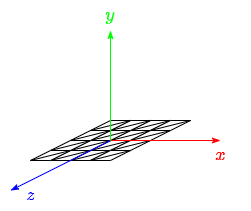
\includegraphics[width=0.25\textwidth]{displacement-0.png} }}
  \qquad
  \subfloat[\centering]{{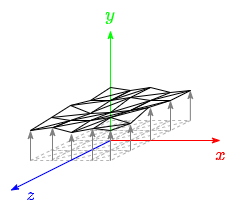
\includegraphics[width=0.25\textwidth]{displacement-1.png} }}%
  \qquad
  \subfloat[\centering]{{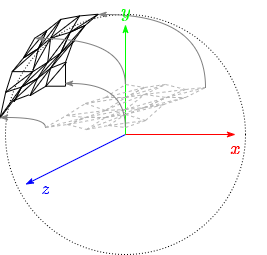
\includegraphics[width=0.25\textwidth]{displacement-2.png} }}%
  \caption{Illustration of what happens to the vertices of a terrain mesh in the terrain mesh vertex shader. 
  Initially, the terrain mesh is lying flat at the null coordinate in subfigure (a).
  In the vertex shader, the height gets sampled from the heightmap texture 
  and the $y$-coordinate of the vertex is displaced as shown in subfigure (b).
  Finally, the vertex is projected to the ellipsoid in subfigure (c).}\label{fig:displacement}
\end{figure}

The pseudocode of the \texttt{main()} function of the vertex shader for the terrain mesh is shown in listing \ref{lst:vertexshadermain}.

\begin{lstlisting}[
  language={C++},
  label={lst:vertexshadermain},
  caption={The \texttt{main()} function for the vertex shader.}]
void main()
{
    float tw = tileWidth - 1;

    // Normalized positions in range [0,1]
    vec2 aPos1 = vec2((aPos.x + 0.5f * tw) / tw,
                        (aPos.y + 0.5f * tw) / tw);

    // Calculate Web mercator Coordinates
    float mercX = (tileKey.x + aPos1.x) / float(1 << int(zoom));
    float mercY = (tileKey.y + aPos1.y) / float(1 << int(zoom));

    // Retrieve height form heightmap (important: denormalize to 255)
    vec3 height = texture(heightmapTexture, aPos1).rgb * 255;

    // Calculate height
    float y = calculateHeight(height);

    // Globe projection
    vec2 lonlat = inverseWebMercator(vec2(mercX, mercY));
    vec3 ellipsoidPos = geodeticToCartesian(globeRadiusSquared, vec3(lonlat.x, y, lonlat.y));

    inTexCoords = aPos1;
    inNormal = geodeticSurfaceNormal(vec3(lonlat.x, y, lonlat.y));
    FragPosition = ellipsoidPos;
    gl_Position = projection * view * model * vec4(ellipsoidPos, 1.0);
}
\end{lstlisting}
For the skirt mesh, the height of a skirt vertex would additionally be subtracted 
by the skirt height after the retrieval of the $y$ value (line 17).

The height calculation occurs with a special scaling in order to account 
for the reduced globe radii as shown in listing \ref{lst:vertexshaderheight}.

\begin{lstlisting}[
  language={C++},
  label={lst:vertexshaderheight},
  caption={The GLSL \texttt{calculateHeight()} function for computing the height value from a RGB triple.}]
  float calculateHeight(vec3 height) {
    // Maptiler Terrain RGB formula
    float y = -10000 + (((height.r * 256.0f * 256.0f * 0.1) + (height.g * 256.0f * 0.1) + (height.b * 0.1)));
    return (y / 20169.51); // Scaling down the Earth radius (globeRadii.x / 6378159.09)
}
\end{lstlisting}

\subsubsection{Fragment Shader}
The fragment shader performs the texturing,
applies an ambient light and the distance fog.
The uniform variable \texttt{useWire} and \texttt{doFog}
signals whether to render in wireframe mode and with fog respectively.
The \texttt{main()} function of the fragment shader is 
shown in listing \ref{lst:fragmain}. The terrain mesh 
and the skirt mesh use essentially the same 
fragment shader code.

\begin{lstlisting}[
  language={C++},
  label={lst:fragmain},
  caption={The \texttt{main()} method for the fragment shader.}]
void main()
{
    vec3 color;
    vec3 lightColor = vec3(1.0f, 1.0f, 1.0f);

   if (useWire < 0.5f) {
       float tw = tileWidth - 1;
       color = texture(overlayTexture, inTexCoords).rgb;
       vec3 ambient = calculateAmbient(lightColor, 0.1f);

       if (doFog > 0.5) {
           vec3 fogColour = vec3(97, 154, 232) / 255.0f;
           float fogFactor = calculateFog(fogDensity);
           color = mix(fogColour, color, fogFactor);
       }
    } else {
        color = terrainColor.rgb;
    }
    FragColor = vec4(color, 1.0f);
}
\end{lstlisting}

The distance fog calculation is partially based on the
the predecessor project \cite{p2} and is shown in listing \ref{lst:fog}:

\begin{lstlisting}[
  language={C++},
  label={lst:fog},
  caption={GLSL pseudocode for the distance fog.}]
float calculateFog(float density) {
    float start = 0.8;
    float end = 3.5;
    float dist = length(cameraPos - FragPosition);
    if (dist < start) return 1.0f;
    float scale = (dist - start) / (end - start);
    float fogFactor = pow(scale, 1);
    return 1.0f - clamp(fogFactor, 0.0f, 0.5f);
}
\end{lstlisting}

\section{Miscellaneous Features}
This section describes some 
miscellaneous features implemented 
in StreamingATLOD.

\subsection{Camera}
The implemented camera is partially based on the chapter ``Camera'' of \textit{Learn OpenGL} by de Vries \cite{learnopengl},
but is slightly modified for Earth rendering.
Moving with the WASD-keys (W for forward, A for left, S for backward, D for right) 
moves the camera in the corresponding 
directions, but in such a way that the Earth stays underneath the camera 
at all times. With the Q and E keys, the altitude can be decreased 
and increased respectively.
 Dragging to the left and right with the mouse
rotates the camera to the left and right, but so 
that the rotation occurs about the vector which goes from 
the closest point on Earth's surface to the camera's position.
Dragging the mouse to the top and bottom rotates 
the camera up and down, with the pitch angle 
being limited to the range of $-89^{\circ}$ to $0^{\circ}$,
so that the camera cannot point directly down towards 
the ground and up towards the sky.
Figure \ref{camera-earth} shows an illustration of the 
Earth-centered camera movement.

\begin{figure}[H]
  \centering
  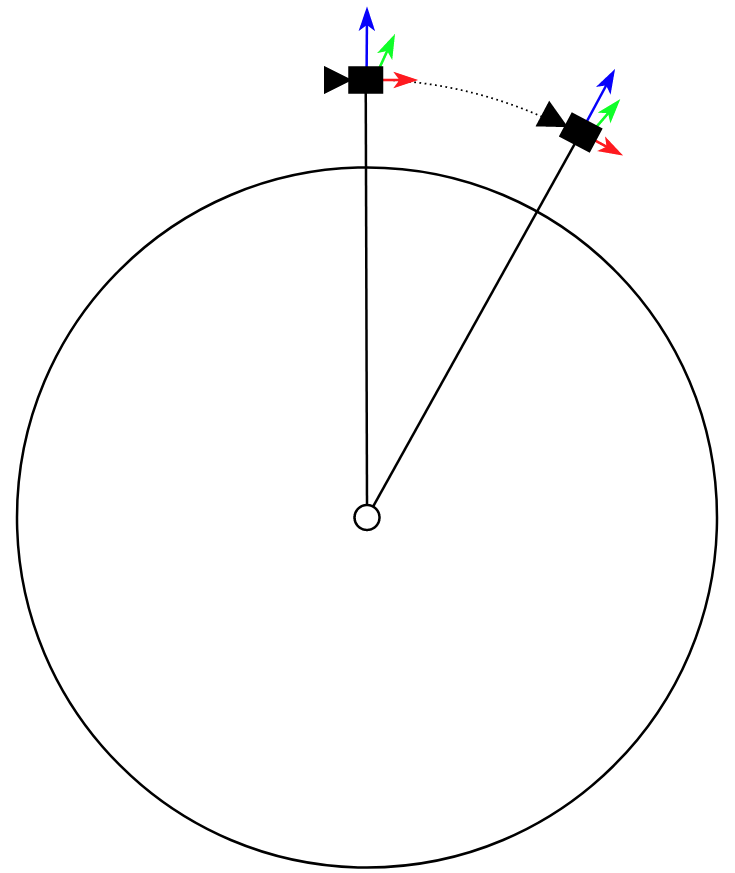
\includegraphics[width=0.4\textwidth]{camera-earth.png}
  \caption{Illustration of the Earth-centered camera. The front vector is red, the right vector green and the up vector blue.}\label{fig:camera-earth}
\end{figure}

Upon keyboard input by the user, we perform the following:
If the camera should move to the left or right, we simply add 
the right vector to the current position and we are done.
Otherwise, if the camera should move up, down, forward or backwards,
we first calculate the Earth's normal vector at the position 
of the camera by taking the length of the camera's position vector,
since the Earth is centered at $(0,0,0)$.
If the camera should move up and down, we multiply the Earth normal vector 
by the velocity and add it to the current position.
If the camera should move forward or backward, we compute a new front vector by projecting the current 
front vector onto the plane orthogonal to the Earth normal. 
Afterwards, we multiply the projected front vector 
by the camera velocity and add the new 
projected front vector to the current position vector.
In addition to the above steps, we limit the camera's position to 
always stay inside a sphere of radius 1000, so that the camera 
doesn't fly away. 

When updating the camera vectors, we first create 
a quaternion \texttt{earthQuat} where the up vector points towards the Earth normal vector.
Afterwards, we first rotate the unit front vector 
according to the Earth with \texttt{earthQuat}, followed by the yaw and pitch rotations.
Afterwards, we normalize the vectors and compute the right and up vectors as well.
Listing \ref{lst:updatecam} shows the 
updating of the camera vectors.

\begin{lstlisting}[
  language={C++},
  label={lst:updatecam},
  caption={Method \texttt{Camera::updateCameraVectors()} that updates the camera vectors.}]
void Camera::updateCameraVectors()
{
    glm::vec3 earthNormal = glm::normalize(_position);

    glm::vec3 earthRight = glm::normalize(glm::cross(earthNormal, _worldUp));
    glm::vec3 earthFront = -1.0f * glm::normalize(glm::cross(earthNormal, earthRight));
    glm::vec3 front1;

    front1 = glm::vec3(0, 0, -1.0);

    glm::mat4 earthMat = glm::mat4(glm::vec4(earthRight, 0),
        glm::vec4(earthNormal, 0),
        glm::vec4(earthFront, 0),
        glm::vec4(0, 0, 0, 1));

    glm::quat pitchQuat = glm::angleAxis(glm::radians(_pitch), earthRight);
    glm::quat yawQuat = glm::angleAxis(glm::radians(_yaw), earthNormal);
    glm::quat earthQuat = glm::quat_cast(earthMat);

    front1 = glm::vec3(yawQuat * pitchQuat * earthQuat * front1);

    _front = glm::normalize(front1);
    _right = glm::normalize(glm::cross(_front, earthNormal));
    _up = glm::normalize(glm::cross(_right, _front));
}
\end{lstlisting}

\subsection{Collision Detection}
The collision detection prevents the camera from 
flying beneath the Earth.
It is implemented using a very simple heightmap check.

First, we need to determine which terrain node's heightmap to use 
for collision detection. We use the following simple observation:
At any point during rendering, the camera is always above 
a single leaf terrain node.

During the collection traversal, when we reach a 
leaf terrain node which should be rendered,
we check whether the camera's longitude and latitude 
is contained inside the terrain node's longitudal 
and latitudal extents. If so, we track the node's tile key 
so that the terrain node can later be used for collision detection.
For checking whether the camera's longitude and latitude 
is contained inside the node's longitude and latitude bounding rectangle,
the camera's position is first transformed to the Web Mercator projection
using \texttt{MapProjections::webMercator()}. The terrain tile's 
corner points are also projected to Web Mercator using the same method.
This updating of the closest tile key is encapsulated in 
the method \texttt{TerrainManager::updateMinimumDistanceTileKey()} 
shown in listing \ref{lst:updateminimumdistancetilekey}.

\begin{lstlisting}[
  language={C++},
  label={lst:updateminimumdistancetilekey},
  caption={Method \texttt{TerrainManager::updateMinimumDistanceTileKey()} that updates the tile key of the minimum distance terrain node.}]
  void TerrainManager::updateMinimumDistanceTileKey(Camera& camera, XYZTileKey currentTileKey, XYZTileKey& minimumDistanceTileKey)
  {
      glm::vec2 cameraLonLat = MapProjections::toGeodetic2D(camera.position(), GlobalConstants::GLOBE\_RADII\_SQUARED);
      glm::vec2 cameraMerc = MapProjections::webMercator(cameraLonLat);
  
      float pow2Zoom = 1 << currentTileKey.z();
      float minMercX = (currentTileKey.x()) / pow2Zoom;
      float maxMercX = (currentTileKey.x() + 1) / pow2Zoom;
      float minMercY = (currentTileKey.y()) / pow2Zoom;
      float maxMercY = (currentTileKey.y() + 1) / pow2Zoom;
  
      // If camera is inside leaf node, update tile key
      if (cameraMerc.x >= minMercX && cameraMerc.x <= maxMercX && cameraMerc.y >= minMercY && cameraMerc.y <= maxMercY)
          minimumDistanceTileKey = currentTileKey;
  }
\end{lstlisting}

After the collection traversal, we compute the local heightmap coordinate 
that we need to retrieve for checking the height value with the camera's height value
and perform the actual collision detection. This is implemented 
in \texttt{TerrainManager::checkCollision()} as shown in listing \ref{lst:checkcollision}.

\begin{lstlisting}[
  language={C++},
  label={lst:checkcollision},
  caption={Method \texttt{TerrainManager::checkCollision()} that performs the collision detection.}]
void TerrainManager::checkCollision(Camera& camera, XYZTileKey minimumDistanceTileKey)
{
    TerrainNode* node = _memoryCache.get(minimumDistanceTileKey).value;
    glm::vec2 lonLat = MapProjections::toGeodetic2D(camera.position(), GlobalConstants::GLOBE_RADII_SQUARED);
    glm::vec2 camMerc = MapProjections::webMercator(lonLat);

    float minDistZoomPow2 = 1 << minimumDistanceTileKey.z();

    // Compute minimum and maximum Web Mercator coordinates.
    float minMercX = (minimumDistanceTileKey.x()) / minDistZoomPow2;
    float maxMercX = (minimumDistanceTileKey.x() + 1) / minDistZoomPow2;
    float minMercY = (minimumDistanceTileKey.y()) / minDistZoomPow2;
    float maxMercY = (minimumDistanceTileKey.y() + 1) / minDistZoomPow2;

    float heightX = ((camMerc.x - minMercX) / (maxMercX - minMercX));
    float heightY = ((camMerc.y - minMercY) / (maxMercY - minMercY));
    glm::vec2 lonLatTerrain = MapProjections::inverseWebMercator(glm::vec2(heightX, heightY));

    verticalCollisionOffset = 0.0;

    // Check if inside bounds
    if (heightX >= 0 && heightX <= 1 && heightY >= 0 && heightY <= 1) {
        // Retrieve height value
        float height = node->getScaledHeight(heightX * 511, heightY * 511);

        // Project height point onto ellipsoid
        glm::vec3 projected = MapProjections::geodeticToCartesian(GlobalConstants::GLOBE_RADII_SQUARED, glm::vec3(lonLatTerrain.x, height + 0.04, lonLatTerrain.y));

        float distCamera = glm::length(camera.position());
        float distHeight = glm::length(projected);

        // Collision
        if (distHeight > distCamera) {
            camera.verticalCollisionOffset(distHeight - distCamera);
        }
    }
}
\end{lstlisting}
First, we transform the camera's world-space coordinates into Web Mercator (lines 4 and 5).
Afterwards, compute the bounding rectangle of the closest node whose tile key is \texttt{minimumDistanceTileKey} (lines 10 to 13).
Next, we compute the heightmap coordinates \texttt{heightX} and \texttt{heightY} 
by normalizing the camera's Web Mercator coordinates (lines 15 and 16) and subsequently compute the 
2D geodetic coordinates \texttt{lonLatTerrain} of the point on the terrain to test (line 17).
We then check whether the \texttt{heightX} and \texttt{heightY} are inside the range $[0,1]$ (line 22)
and if so, retrieve the height value by scaling \texttt{heightX} and \texttt{heightY} by 
the image width and height respectively and calling \texttt{TerrainNode::getScaledHeight()} (line 24).
With the newly retrieved height value plus a small offset value and \texttt{lonLatTerrain}, we compute the actual terrain
point in cartesian coordinates to compare with the camera position (line 27).
Since the Earth is centered around $(0,0,0)$, if suffices to compare the length of both vectors (lines 29 and 30).
If the position of the terrain point is higher than the camera's position, we set the vertical collision offset value in 
the camera (lines 33 and 34) such that it can later correct the offset and thus not fly under the Earth.

\subsection{Skybox}
Currently, StreamingATLOD uses a simple 
cubemap for rendering the sky. The implementation of the cubemap 
is based on chapter ``Cubemaps'' from \textit{Learn OpenGL} by de Vries \cite{learnopengl}.
At runtime, the skybox is rotated such that it always points in the direction of the normal vector of the 
Earth relative to the camera, such that the blue sky always points upwards.

\subsection{Application Configuration}
StreamingATLOD can be configured using a 
configuration file named \texttt{config.txt}.
The configuration file consists of simple key-value pairs
per line, with the key and value delimited by an equal symbol (=).
The following options must be set:
\begin{itemize}
  \item Heightmap service URL: The URL for the heightmap web API.
  \item Overlay service URL: The URL for the overlay web API.
  \item Heightmap service key: The key for the heightmap web API.
  \item Overlay service key: The key for the overlay web API.
  \item Maximum zoom level: The maximum zoom level a terrain node can reach. Limited to between 0 and 30. Setting this value higher than what the APIs can serve risks making unnecessary API requests.
  \item Memory cache size: The maximum number of elements in the memory cache. Limited to between 100 and 500.
  \item Disk cache size: The maximum number of elements in the disk cache. Limited to between 400 and 8000. Also, the disk cache capacity must be at least four times the memory cache capacity.
  \item Disk cache location: The location of the disk cache on the file system.
  \item Number of load workers: The number of load worker threads. Limited to between 1 and 8.
  \item Low resolution mesh size: The side length of the low resolution terrain mesh. Limited to between 8 and 512.
  \item Medium resolution mesh size: The side length of the medium resolution terrain mesh. Limited to between 8 and 512.
  \item High resolution mesh size: The side length of the high resolution terrain mesh. Limited to between 8 and 512.
  \item Data folder location: The location of the data folder, which contains the GLSL shader code and skybox images.
\end{itemize}

The configuration file is loaded and validated at startup
and is managed as a singleton class \texttt{ConfigManager}.
After the loading of the configuration file, the 
configuration settings stay constant throughout the runtime of StreamingATLOD and are not
changed.

The details on how to set configurations and launch StreamingATLOD with them 
are described in the \texttt{README} of StreamingATLOD's GitHub repository\footnote{\url{https://github.com/amartabakovic/bachelor-thesis}}.

\subsection{Debug Visualizations}
Various minor debug visualizations were implemented 
in order to showcase how the various implemented techniques work.

\subsubsection{Camera Freezing}
Freezing the camera means that the logical camera (i.e. the position and front vectors and the view-frustum) 
get frozen in place, while the actual camera can still be flown around. 
With a frozen camera, the culling techniques and the LOD calculation get forzen in place as well.
For this, the application always keeps track of two varaibles: \texttt{Camera oldCamera} and \texttt{Camera camera}.
Every frame, \texttt{oldCamera} is set to \texttt{camera} and subsequently
\texttt{oldCamera} is passed to the \texttt{TerrainManager::render()} method.
If the user activates camera freezing, then \texttt{oldCamera} is no longer updated to be \texttt{camera}.
This means that \texttt{TerrainManager::render()} continues to compute culling and LOD with \texttt{oldCamera},
while \texttt{camera} is used for the camera movement and the model-view-projection matrix.
Figure \ref{fig:freeze} shows an example of camera freezing.

\begin{figure}[H]
  \centering
  \subfloat[\centering]{{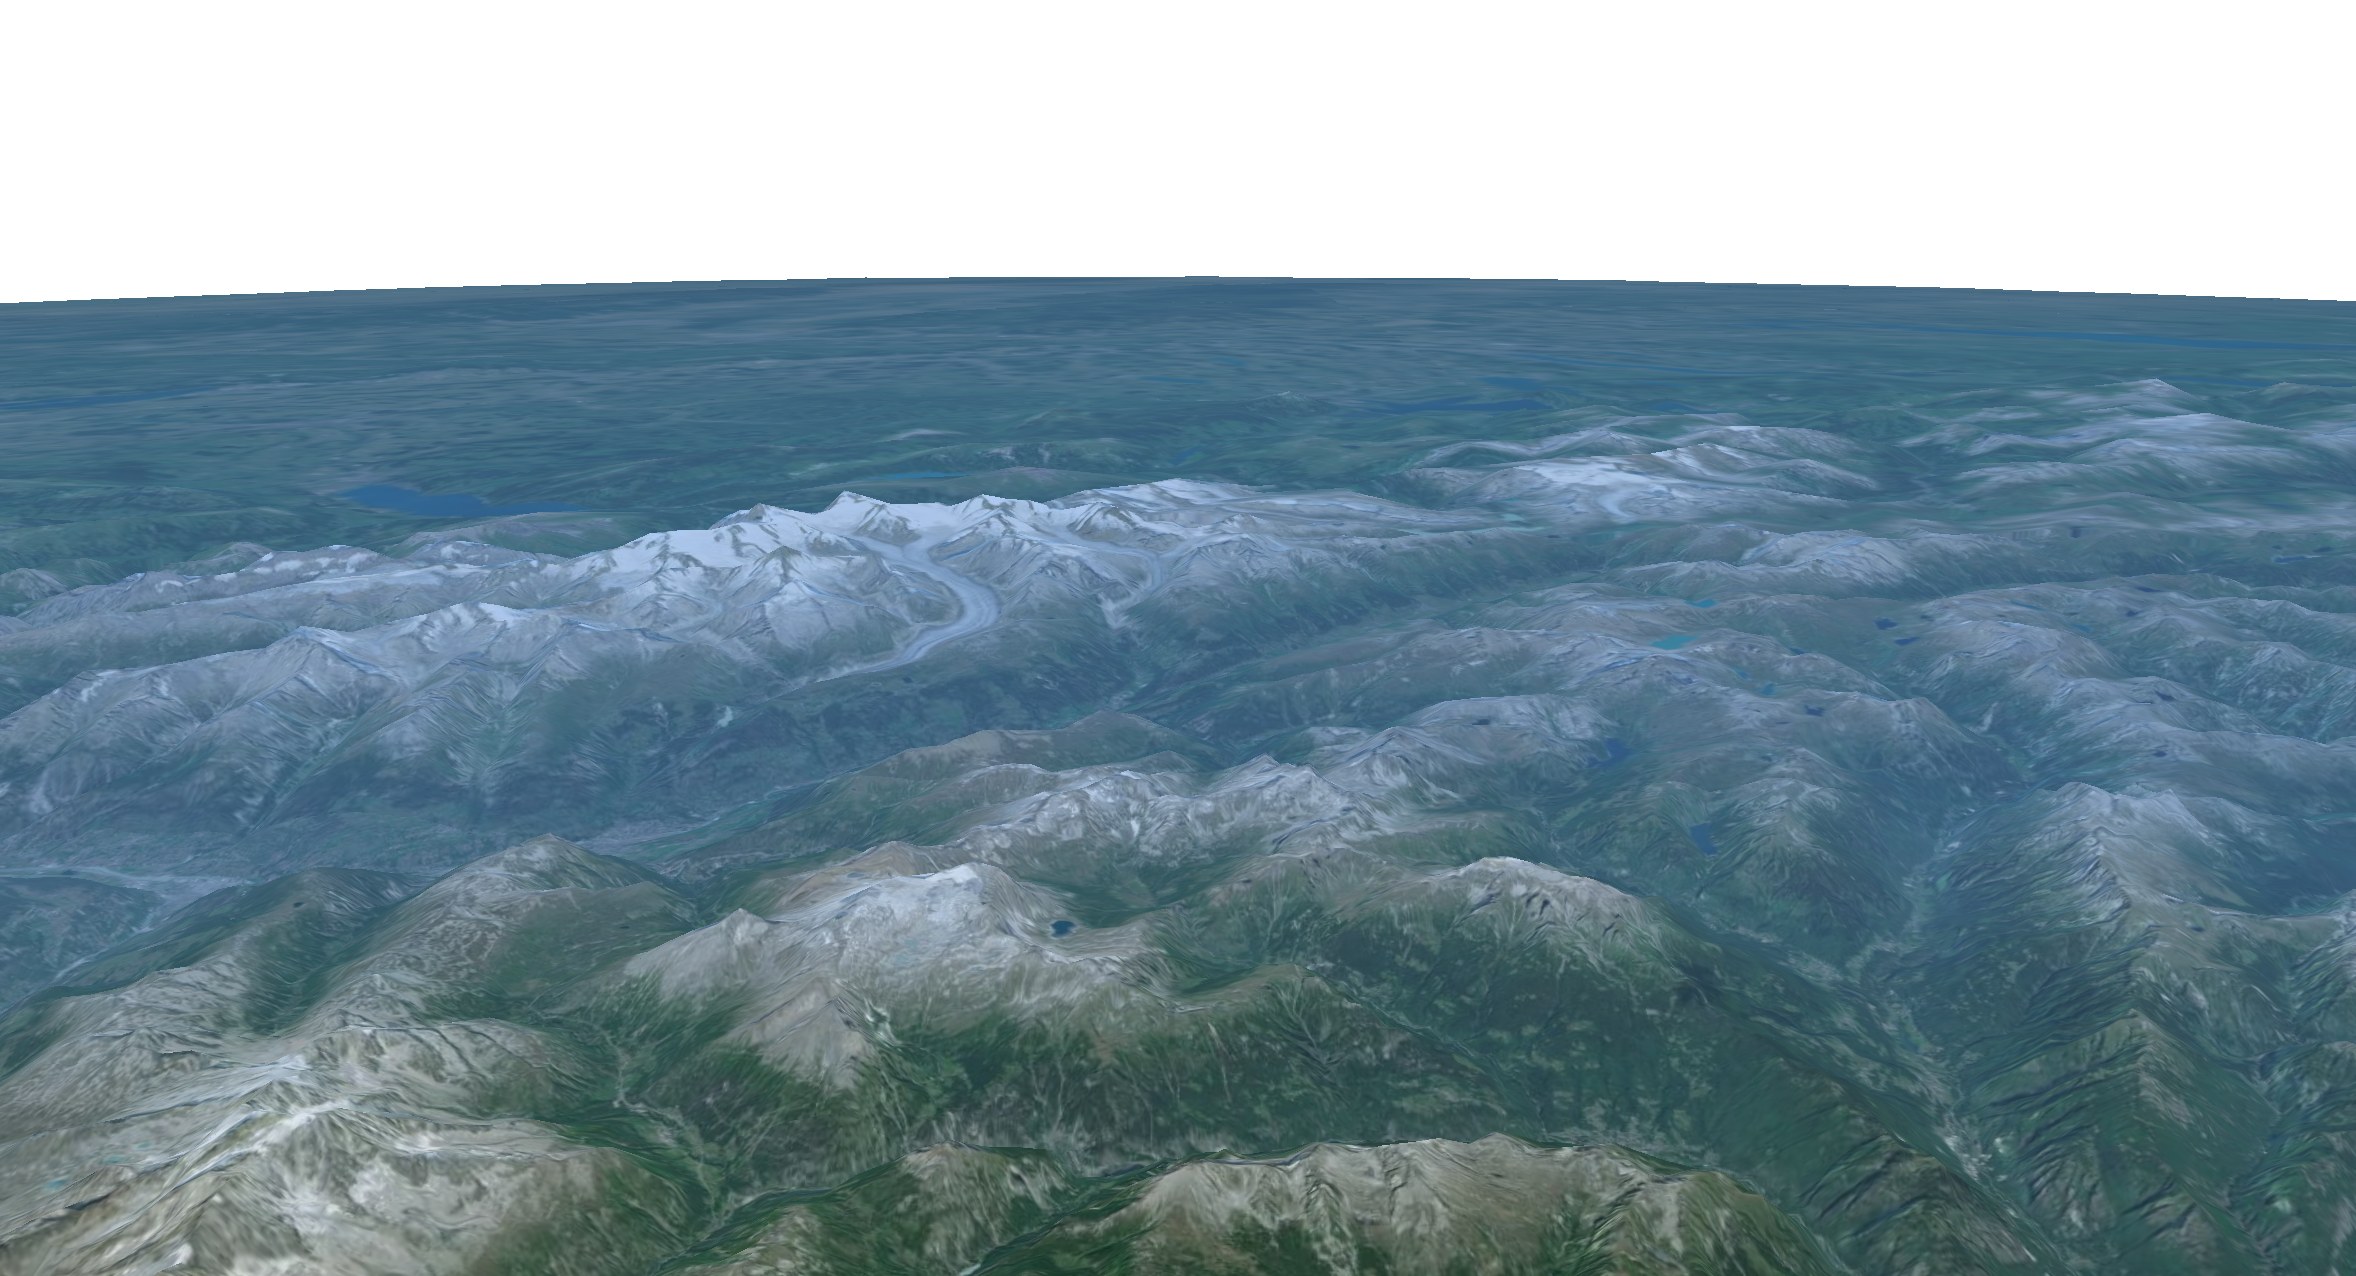
\includegraphics[width=0.4\textwidth]{before-freeze.png}}}
  \qquad
  \subfloat[\centering]{{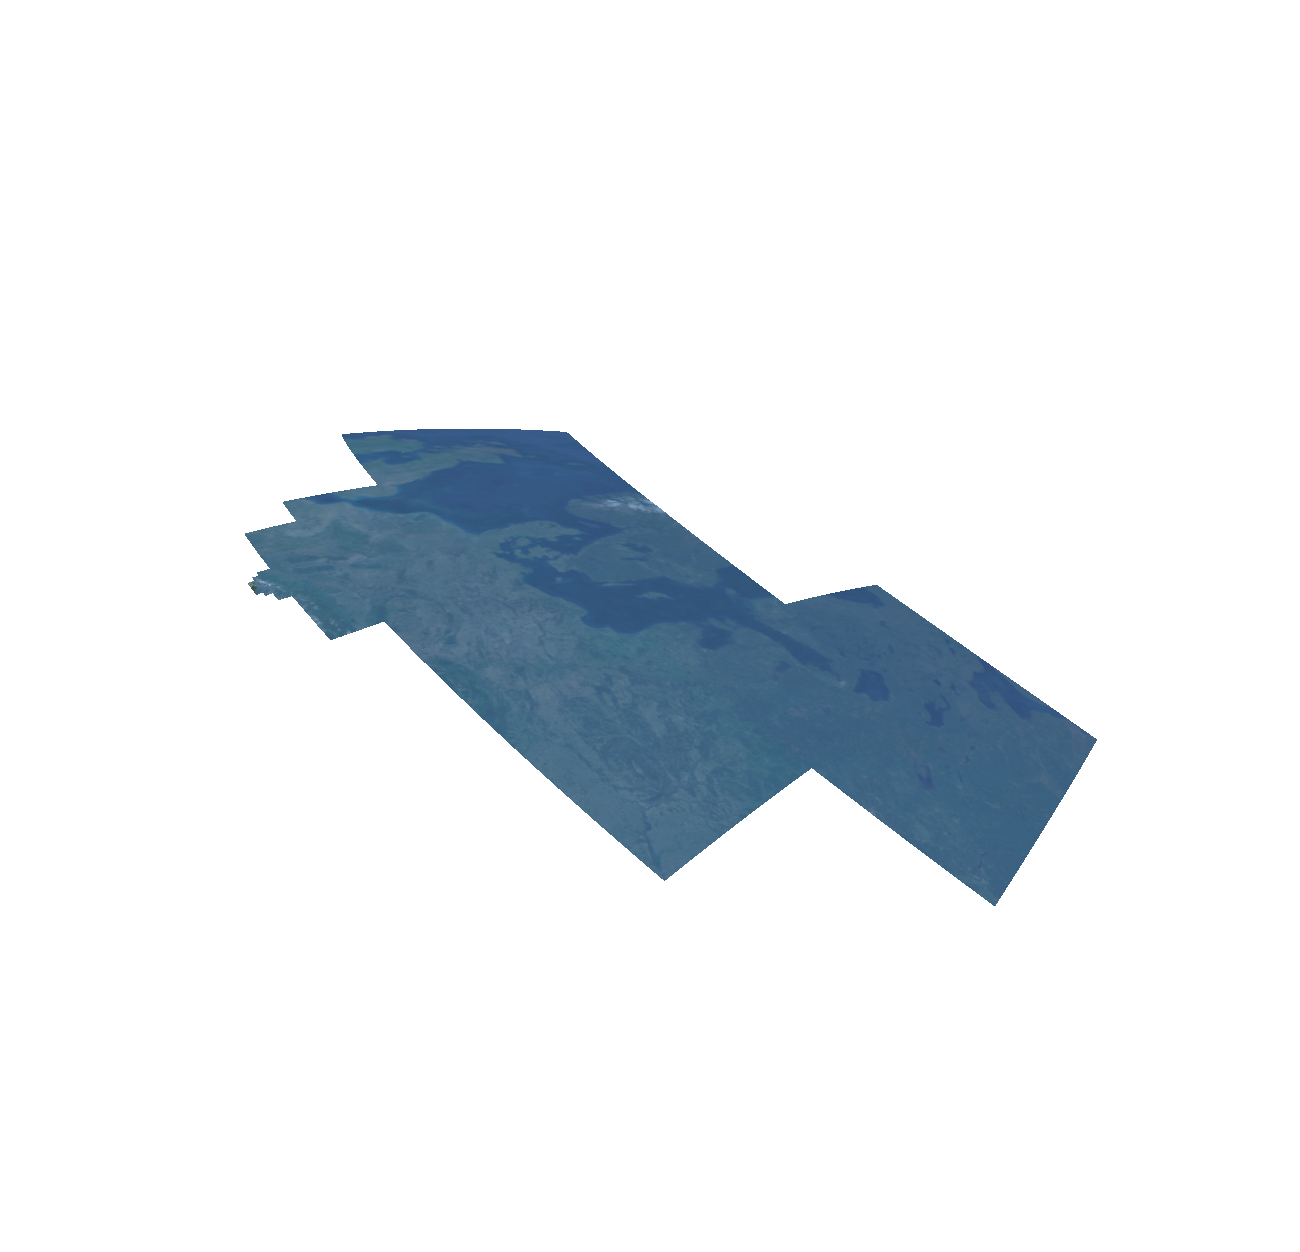
\includegraphics[width=0.4\textwidth]{after-freeze.png} }}%
  \caption{The view from the frozen camera shown in subfigure (a) what actually gets rendered as from the frozen camera in subfigre (b).}\label{fig:freeze}
\end{figure}

\subsubsection{Rendering AABBs}
For rendering AABBs, there is an \texttt{AABBMesh} class and a corresponding shader consisting of \texttt{aabbmesh.vert}
and \texttt{aabbmesh.frag}. The AABB mesh, like the terrain, skirt and pole meshes, is defined once 
during startup and stored as a member in \texttt{TerrainManager}.
During rendering, the AABB is scaled and translated using the terrain node's minimum and maximum points.

An example of an AABB render is shown in figure \ref{fig:debug-aabb}.

\begin{figure}[H]
  \centering
  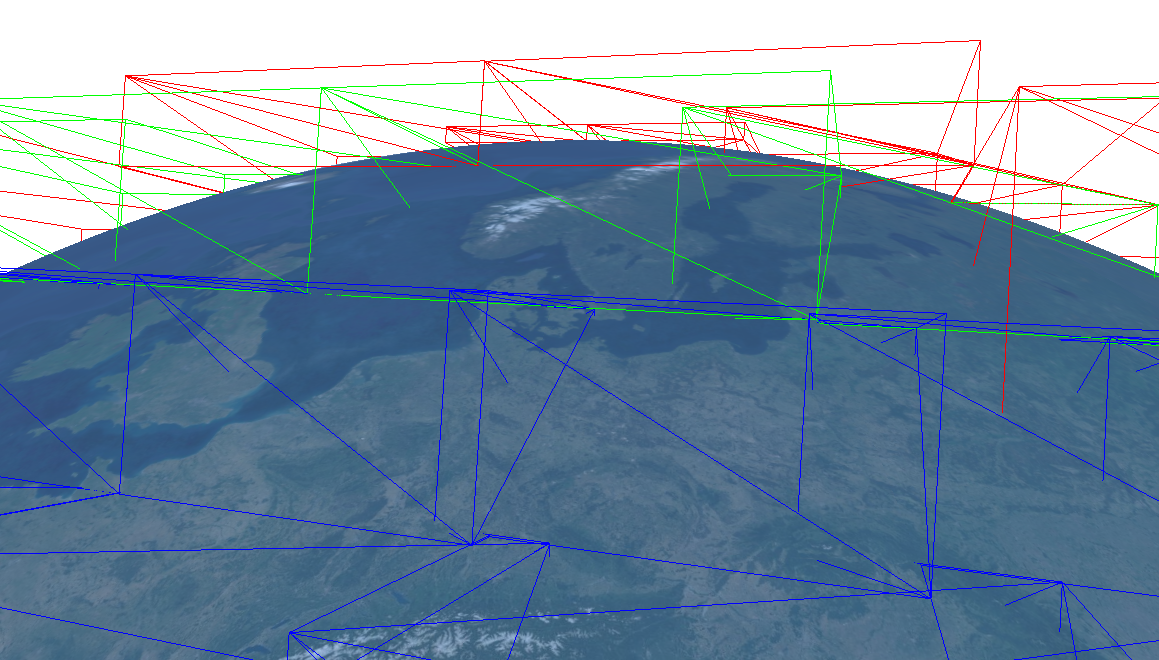
\includegraphics[width=1\textwidth]{debug-aabb.png}
  \caption{Screenshot of a debug AABB render.}\label{fig:debug-aabb}
\end{figure}

\subsubsection{Wireframe Mode}
The wireframe of the terrain is rendered using the OpenGL command \texttt{glPolygonMode(GL\_FRONT\_AND\_BACK, GL\_LINE)}.
Prior to the draw call, the uniform \texttt{vec3} variable \texttt{terrainColor} of the terrain shader is set to either red,
green or blue, according to the following listing:

\begin{lstlisting}[
  language={C++},
  label={lst:render},
  caption={Setting the color of the terrain for the wireframe mode.}]
// Set colors for debug wireframe view
glm::vec3 terrainColor = glm::vec3(1, 0, 0);
if (wireframe) {
    if (zoom % 3 == 1)
        _terrainShader.setVec3("terrainColor", glm::vec3(0, 1, 0));
    else if (zoom % 3 == 2)
        _terrainShader.setVec3("terrainColor", glm::vec3(0, 0, 1));
}

_terrainShader.setVec3("terrainColor", terrainColor);
\end{lstlisting}

An example of a wireframe render is shown in figure \ref{fig:debug-wireframe}.

\begin{figure}[H]
  \centering
  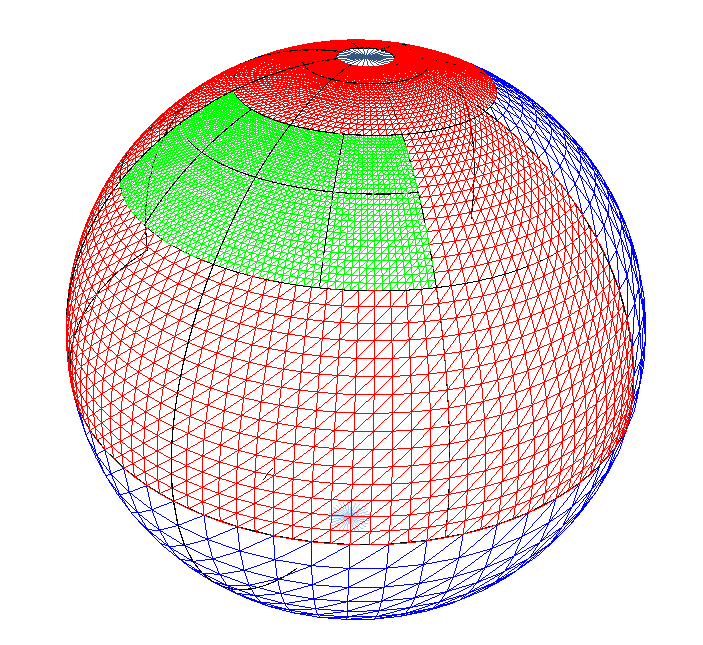
\includegraphics[width=0.5\textwidth]{debug-wireframe.png}
  \caption{Screenshot of a debug wireframe render.}\label{fig:debug-wireframe}
\end{figure}
